\documentclass[a4paper,12pt]{article} % A4, шрифт 12pt
\usepackage[left=30mm, right=15mm, top=20mm, bottom=20mm]{geometry} % Поля
\usepackage{setspace}  % Для изменения межстрочного интервала
\onehalfspacing  % Межстрочный интервал 1.5
\usepackage{indentfirst}  % Красная строка в первом абзаце секции
\setlength{\parindent}{1.25cm}  % Абзацный отступ 1.25 см

\usepackage[T2A]{fontenc}			
\usepackage[utf8]{inputenc}			
\usepackage[english,russian]{babel}	


\usepackage{amsmath,amsfonts,amssymb,amsthm,mathrsfs,mathtools} 
\usepackage{cancel}
\usepackage{multirow}
\usepackage[colorlinks, linkcolor = blue]{hyperref}
\usepackage{upgreek}
\usepackage{graphicx,wrapfig}
\usepackage{bm}
\usepackage{float}
\usepackage[table]{xcolor} % убран xcdraw
\usepackage{tikz}
\usepackage{pgfplots}
\graphicspath{{pictures/}}

\usepackage[sorting=none,backend=biber,style=gost-numeric]{biblatex}
\addbibresource{references.bib}


\usepackage{graphicx}
\usepackage{subcaption}

\usepackage{booktabs}
\usepackage{algorithm}
\usepackage{algpseudocode}

\usepackage{todonotes} 
\reversemarginpar
\setlength{\marginparwidth}{2.5cm}

\usepackage[acronym]{glossaries}

\makeglossaries


\newacronym[
	first={Agent-based model (агентная модель)},
	firstplural={Agent-based models (агентные модели)}
]{abm}{ABM}{Agent-based model (агентная модель)}

\newacronym{sir}{SIR}{susceptible $\rightarrow$ infectious $\rightarrow$ recovered (восприимчивый $\rightarrow$ инфицированный $\rightarrow$ восстановившийся)}

\newacronym{sis}{SIS}{susceptible $\rightarrow$ infectious $\rightarrow$ susceptible (восприимчивый $\rightarrow$ инфицированный $\rightarrow$ восприимчивый)}

\newacronym{seir}{SEIR}{susceptible $\rightarrow$ exposed $\rightarrow$ infectious $\rightarrow$ recovered (восприимчивый $\rightarrow$ подверженный $\rightarrow$ инфицированный $\rightarrow$ восстановившийся)}

\newacronym{covasim}{\texttt{Covasim}}{COVID-19 Agent-based Simulator (агентный симулятор COVID-19)}

\newacronym{covid}{COVID-19}{Coronavirus Disease 2019 (коронавирусная инфекция 2019)}

\newacronym{sars}{SARS-CoV-2}{Severe acute respiratory syndrome-related coronavirus 2 (коронавирус 2, связанный с тяжелым острым респираторным синдромом)}

\newacronym{gil}{GIL}{Global Interpreter Lock (глобальная блокировка интерпретатора)}


\begin{document}

\begin{titlepage}

\begin{center}
    {\large Федеральное государственное автономное 
образовательное учреждение высшего образования 
«Московский физико-технический институт 
(национальный исследовательский университет)»}
\end{center}
\begin{center}
    {\large Физтех-школа биологической и медицинской физики \\ Кафедра системной и синтетической биологии}
\end{center}
\noindent \textbf{Направление подготовки:} 03.03.01 Прикладные математика и физика

\noindent \textbf{Направленность (профиль) подготовки:} Системная и синтетическая биология

    \vspace{3.5cm}


\vspace{0.1cm}
{\huge
\begin{center}
    \textbf{Исследование роли транспортных потоков в развитии эпидемии на основе компьютерной агентной модели}
   \\
\end{center}
}
{\large
\begin{center}
    (бакалаврская работа)
   \\
\end{center}
}
\vspace{3.5cm}

\begin{flushright}
\large \textbf{Студент:} \\Клочков Константин Александрович
\vspace{0.2cm}
\end{flushright}

\begin{flushright}
\large \textbf{Научный руководитель:} \\ Манолов Александр Иванович, \\ к.б.н
\vspace{0.2cm}
\end{flushright}

\vspace{2.5cm}

\begin{center}
    Москва 2025
\end{center}

\end{titlepage}

\section*{Аннотация}
В данной работе мы исследовали роль транспортных потоков в распространении эпидемии на основе агентной модели Covasim.

Была реализована возможность моделирования пассажиропотоков (обмена агентами между населенными пунктами), добавлена опция введения ограничений на передвижение, а также изучено влияние уровня заразности инфекционного агента и конфигурации транспортной сети на развитие эпидемического процесса.

В ходе исследования были изучены характер зависимости смещения пика эпидемиологической кривой от интенсивности транспортного потока, чувствительность различных эпидемических метрик к изменению входящих и исходящих потоков, а также возможность идентификации населенного пункта, в котором началась эпидемия.

Кроме того, продемонстрирована значимость своевременного ограничения транспортных потоков для снижения нагрузки на систему здравоохранения — на примере распространения вируса SARS-CoV-2.

%В данной работе на основе высокопроизводительной агентной модели были созданы модели системы двух городов, системы хаб-сателлиты и внутрироссийских авиаперелетов. По результатам их исследования были определены характер зависимости смещения пика эпидемиологической кривой от величины транспортного потока, чувствительность различных метрик эпидемии к изменению входящего и исходящего потоков, возможность детектирования города начала. Также была продемонстрирована важность своевременного ограничения этих потоков для значительного снижения нагрузки на систему здравоохранения на примере распространения уханьского варианта SARS-CoV-2.

\newpage

\section*{Список сокращений}
%\printacronyms[name={}]
\printglossary[type=\acronymtype, title={}]
\newpage

\tableofcontents
\newpage



\section{Введение}
С увеличением вычислительных мощностей математические модели стали важнейшими инструментами анализа распространения инфекционных заболеваний и поиска способов борьбы с ними \cite{hethcote2000mathematics, hethcote1989three, hethcote1992transmission}. Агентные модели при наличии достаточных объемов демографических данных способны описать развитие эпидемии на уровне отдельных агентов (людей), что позволяет рассматривать сложные социальные структуры, динамические изменения в них, иммунологическую историю индивидов и многие другие особенности, недоступные детерминистическим компартментным моделям, основанным на дифференциальных уравнениях \cite{rakowski2010influenza}.

Целью данной работы является исследование влияния транспортных потоков и ограничений, накладываемых на них, на ход протекания эпидемии в модельных системах на основе высокопроизводительной агентной модели.

Исследования в рамках данной работы проводились на модели, разработанной нами ранее на основе \gls{covasim}. \gls{covasim} — агентная модель с открытым исходным кодом, содержащая реалистичную систему передачи инфекции в разных социальных слоях и протекания болезни, зависящую от возраста агента \cite{kerr2021covasim}.

Мы внедрили в \gls{covasim} модель транспортных потоков: вычисления, соответствующие различным населенным пунктам, ведутся параллельно. На каждом шаге симуляции в каждом городе выбираются случайные агенты-туристы, количество которых согласуется с величинами транспортных потоков. Агент-турист удаляется из сети контактов своего населенного пункта и внедряется в город прибытия, вступая в фиксированное число случайных контактов. По завершении периода поездки производится обратная операция. Перемещениям не подвержены агенты в тяжелом или критическом состоянии: если они оказываются в списке туристов, то не покидают свой город. Если же они оказались в таком состоянии по завершении периода поездки, они возвращаются в родной город только при выздоровлении.

Данная работа демонстрирует важность транспортных потоков и своевременного их ограничения в развитии эпидемии. В дальнейшем планируется исследовать распространение \gls{sars} и других менее трансмиссивных заболеваний в случае туристических поездок по Российской Федерации.


\section{Обзор литературы}
\subsection{Виды эпидемиологических моделей}

Математические модели стали важными инструментами анализа распространения инфекционных заболеваний и способов борьбы с ними. В процессе создания модели уточняются предположения и параметры. Само же моделирование позволяет оценить критические значения параметров модели, приводящие к развитию эпидемии: базовый индекс репродукции инфекции $R_0$, эффективный $R_{\text{eff}}$, среднее число контактов между людьми. Математические модели и компьютерное моделирование являются полезными экспериментальными инструментами для проверки теорий, оценки количественных гипотез, ответов на конкретные вопросы, определения чувствительности к изменениям значений параметров и оценки ключевых параметров по данным. Понимание особенностей передачи инфекционных заболеваний в сообществах, регионах и странах может привести к улучшению подходов к снижению распространения этих заболеваний. Математические модели используются при сравнении, планировании, реализации, оценке и оптимизации различных методов
программ по выявлению, профилактике, лечению и контролю. Моделирование в эпидемиологии может способствовать разработке и анализу эпидемиологических обследований, предлагать важнейшие данные которые необходимо собрать, выявить тенденции, сделать общие прогнозы и оценить неопределенность прогнозов \cite{hethcote2000mathematics, hethcote1989three,hethcote1992transmission}.

\subsubsection{Детерминистические компартментные модели}

Подавляющее большинство эпидемиологических моделей основано на компартментализации людей или иных моделируемых сущностей в зависимости от их состояния \cite{keeling2005networks,kermack1927contribution,bailey1957mathematical,anderson1992may}. Базовые модели описывают лишь два компартмента: восприимчивых и инфицированных. В таком случае происходит пренебрежение многими деталями развития эпидемии, тем не менее такие модели все еще активно применяются. Такая \gls{sis} модель описывается системой дифференциальных уравнений
\begin{equation}
    \left\{
    \begin{aligned}
        & \frac{dS}{dt} = gI-\lambda S, \\
        & \frac{dI}{dt} = \lambda S - gI,
    \end{aligned}
    \right.
\end{equation}
другой из основных используемых является \gls{sir} модель, в которой вводится третий компартмент восстановившихся
\begin{equation}
    \left\{
    \begin{aligned}
    & \frac{dS}{dt}=bN-\lambda S-dS, \\
    & \frac{dI}{dt}=\lambda S-gI-dI, \\
    & \frac{dR}{dt}=gI-dR.
    \end{aligned}
    \right.
\end{equation}

Переменные $S$, $I$, $R$ обозначают количества восприимчивых, инфицированных, восстановившихся людей соответственно; $N$ --- размер популяции; $b$, $d$, $g$ --- коэффициенты рождаемости, смертности и восстановления (доля рождающихся, умирающих, восстанавливающихся людей в единицу времени); $\lambda$ --- сила инфекции (доля восприимчивых людей, инфицируемых в единицу времени).

\gls{sir} модели применяются для описания инфекционных заболеваний, формирующих очень стойкий или пожизненный иммунитет, например, кори, коклюша \cite{keeling2005networks,kermack1927contribution,anderson1992may,grenfell1992chance,rohani2000impact}. \gls{sis} модели используют преимущественно при описании распространения заболеваний, передающихся половым путем, реинфицирование которыми вполне возможно, например, хламидиоза, гонореи \cite{keeling2005networks,hethcote1984springer,garnett1996sexually}.

Также активно применяются модифицированные модели с уточненной компартментализацией для более сложного протекания болезни \cite{keeling2005networks, anderson1988epidemiology, grenfell2001travelling} и с более проработанной структурой популяции \cite{hethcote1984springer, ghani1997role, keeling1997modelling}.


%\begin{figure}[]
%    \centering
%    \begin{subfigure}{0.45\linewidth}
%        \centering
%        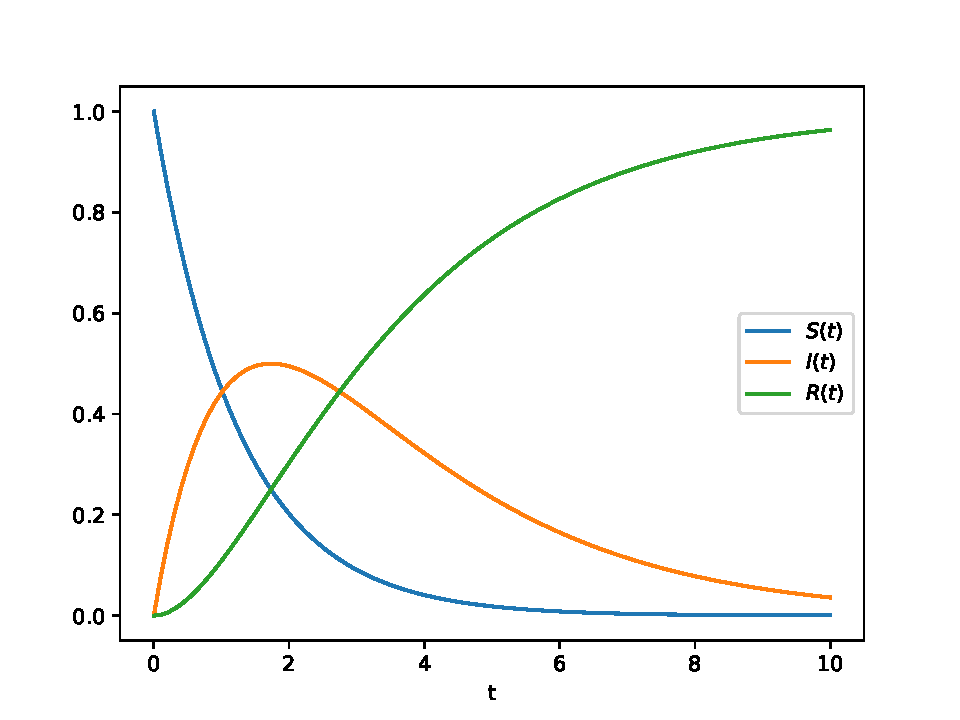
\includegraphics[width=\linewidth]{images/sir.pdf}
%        \caption{\gls{sir} модель}
%    \end{subfigure}
%    \hfill
%    \begin{subfigure}{0.45\linewidth}
%        \centering
%        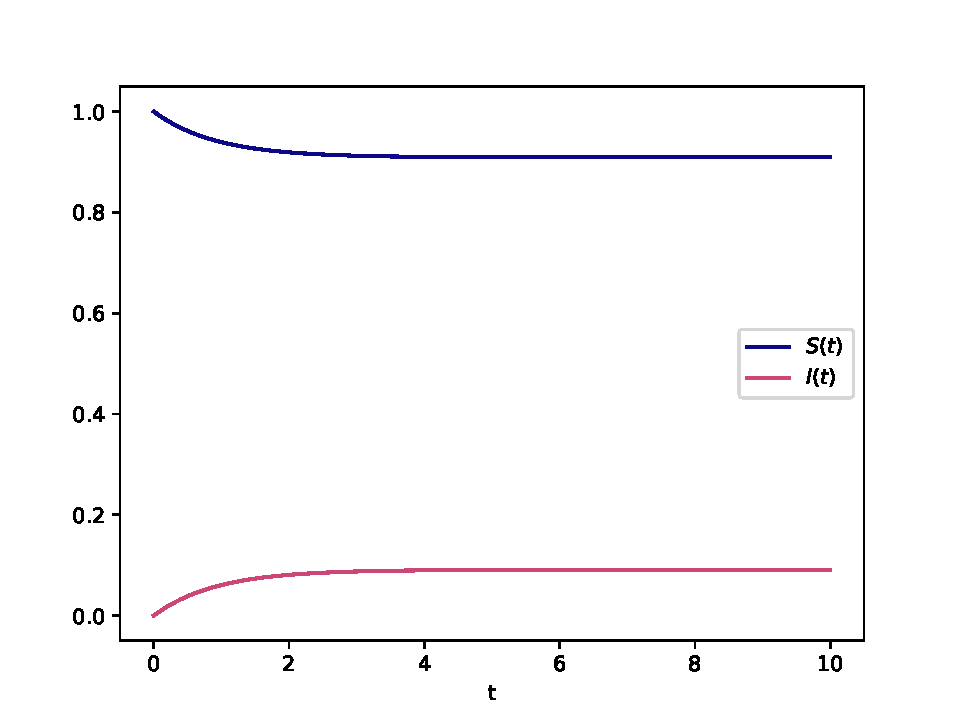
\includegraphics[width=\linewidth]{images/sis.pdf}
%        \caption{\gls{sis} модель}
%    \end{subfigure}
%    \caption{Численные решения задачи Коши компартментных моделей с начальными условиями %$S(0)=1$, $I(0)=0$, $R(0)=0$ и параметрами $b=d=0$, $g=0.4$, $\lambda=0.8$, $N=1$}
%\end{figure}

\begin{figure}[]
    \centering
    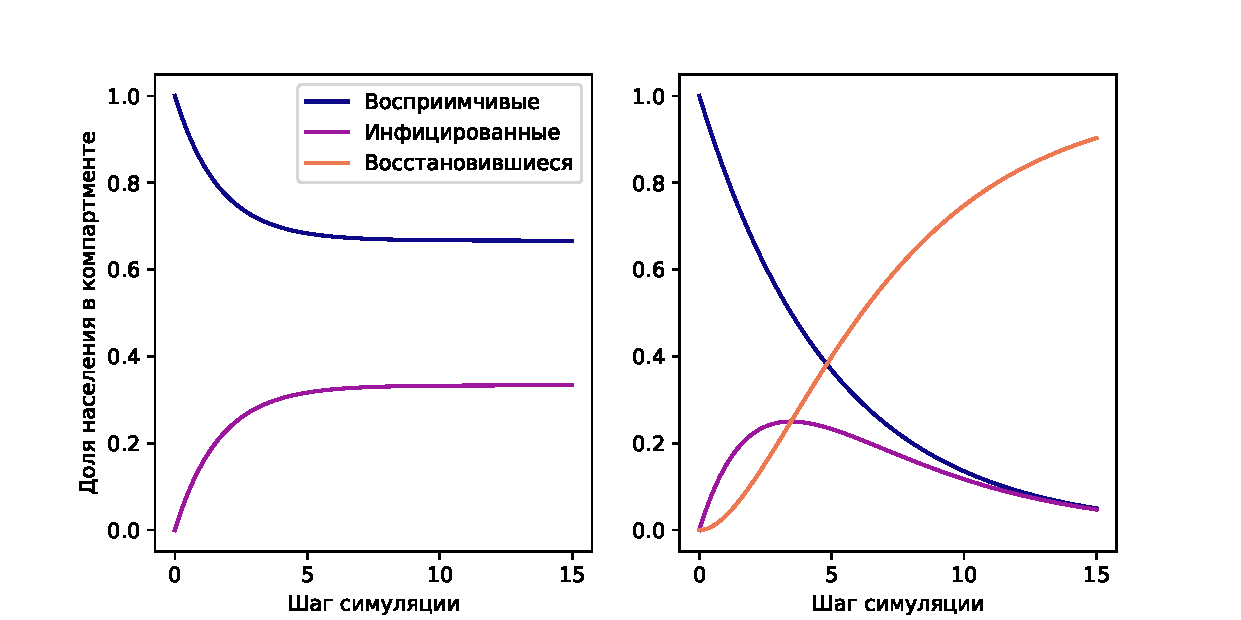
\includegraphics[width=\linewidth]{images/compartment.pdf}
    \caption{Численные решения задачи Коши компартментных моделей с начальными условиями $S(0)=1$, $I(0)=0$, $R(0)=0$ и параметрами $b=d=0$, $g=0.4$, $\lambda=0.2$, $N=1$: слева для \gls{sis} модели, справа для \gls{sir}.}
\end{figure}


\subsubsection{Детерминистические модели среднего поля}
Компартментные модели строятся в предположении, что каждый человек взаимодействует с каждым. Однако в большой популяции у каждого индивида есть свой ограниченный круг общения. Именно им определяется путь распространения инфекции, причем число контактов очень сильно меняется от человека к человеку \cite{pastor2001epidemic}. Для более реалистичного описания таких социальных взаимодействий распространение эпидемии моделируют на графе контактов (или сети контактов). В нем каждому человеку соответствует узел, а каждой социальной связи --- ребро графа \cite{sherborne2018mean}.

В связи с тем, что прямой анализ стохастического поведения эпидемии на графе является сложным, его описывают детерминистическим приближением среднего поля. Анализируют некоторые средние характеристики моделей \cite{sherborne2018mean}. Другими словами, в таких моделях для упрощения математического описания вводятся различные приближения: попарные модели рассматривают состояния пар узлов, соединенных ребром \cite{keeling1999effects, house2011insights}; message passing (обмен сообщениями) (MP) модели рассматривают каждый узел и все возможные пути передачи инфекции в этот узел независимо \cite{karrer2010message}; модели средней степени вершины графа учитывают звездчатые структуры --- узлы с их соседями с учетом их состояния \cite{lindquist2011effective}; edge-based compartmental models (компартментные модели на ребрах графа) (EBCM) оценивают вероятность случайного узла остаться восприимчивым \cite{miller2012edge}. Все эти модели можно построить на одном и том же графе контактов, исходя из разных предположений. При этом часть из них оказывается эквивалентна друг другу \cite{sherborne2018mean}.

Эти модели лучше описывают социальное устройство популяции, однако они рассматривают марковский процесс. Они исходят из предположения, что состояние графа на следующем шаге определяется лишь его состоянием на текущем шаге и никак не зависит от предыдущих шагов. Эти предположения часто оказываются неверны, так как инфицирование или выздоровление происходит не случайно в любой момент времени, а после конкретного инкубационного периода или периода болезни соответственно \cite{keeling2005networks,volz2008sir,house2011insights}. 

\subsubsection{Моделирование при помощи марковских цепей}
Результатами применения марковских цепей также являются временные зависимости некоторых глобальных величин \cite{aiello2003new,haas1999temporal}. Однако, в отличие от детерминистических моделей, стохастический подход допускает временные флуктуации как на глобальном уровне, так и на локальном --- флуктуации на уровне агентов в зависимости от их контактов \cite{nakamura2017efficient}.

Основой таких моделей, как и с моделями среднего поля, часто является граф взаимодействий, описываемый матрицей контактов \cite{albert2002statistical}. В отличие от компартментных детерминистических моделей, матрица контактов может содержать в себе крайне сложные социальные структуры. Это позволяет наблюдать более широкий спектр эпидемиологических явлений \cite{pastor2015epidemic}. Распространение инфекции задается матрицей перехода $\hat{T}$, матричные элементы $T_{\mu\nu}$ которой равны вероятностям перехода из состояния графа $\nu$ (конфигурации всех узлов) в $\mu$ \cite{van1992stochastic}. Эта разница между детерминистическими компартментными моделями и моделями на марковских цепях приводит к различию между временными зависимостями эпидемиологических статистик. К примеру, оказывается, что, хоть \gls{sis} модель демонстрирует схожее с аналогичной стохастической поведение при различных соотношениях между силой инфекции и коэффициентом восстановления, на ранних этапах развития эпидемии, когда среднее число инфицированных сильно меньше размера популяции, ключевым фактором являются именно флуктуации числа инфицированных. И именно такому режиму соответствуют санитарные меры по сдерживанию эпидемий на ранних стадиях \cite{nakamura2017efficient}.

\subsubsection{Агентные модели}
Агентные модели (agent-based models) (\glslink{abm}{ABMs}) применяются при моделировании распространения инфекционных заболеваний уже более 40 лет \cite{fox1971herd, elveback1976influmza}, однако из-за недостатка данных и вычислительных мощностей раскрывать свой потенциал они начали совсем недавно \cite{koopman2002controlling}.

Устройство \gls{abm} позволяет напрямую описывать сложные социальные и физические системы. Хоть для воспроизведения социальной структуры конкретной страны или города может потребоваться очень много данных, \gls{abm} может отразить неоднородность социальных взаимодействий и динамические изменения в структуре сети \cite{rakowski2010influenza}. 

Такой подход очень полезен для реализации учета иммунологической истории индивидов, вариации климата между регионами, социальных структур, что позволяет проводить более тонкую калибровку. Также \gls{abm} позволяют рассматривать распространение инфекции в маленьких группах людей \cite{rakowski2010influenza}.

Типичное построение \gls{abm} требует, во-первых, воссоздания искусственной популяции, соответствующей демографическим данным в регионе, и, во-вторых, создания сети публичных объектов, таких как школ, рабочих мест, где агенты могут взаимодействовать друг с другом. Главной сложностью при построении достаточно подробной \gls{abm} является тот факт, что требуемая информация часто скрыта при агрегировании федеральными службами государственной статистики. В связи с этим возникает необходимость в разработке методов, позволяющих оценить исходные данные из агрегатов, или моделей, приближающих искомые данные \cite{rakowski2010influenza}. 

\subsection{Подходы к изучению транспортных потоков в эпидемиологии}
Транспорт играет важнейшую роль в жизни людей и в то же время активно способствует распространению эпидемий. В связи с этим введение ограничений на транспортные потоки является важной противоэпидемической мерой \cite{li2021modeling}, а понимание влияния этих мер позволит человечеству эффективнее бороться с распространением инфекционных заболеваний.

В имеющихся исследованиях по этой теме транспорт описывается преимущественно детерминистическими компартментными моделями, марковскими моделями на графах и агентными моделями. Статистические (регрессионные и авторегрессионные модели на пространственных данных) же для этих целей практически не применяются в связи с необходимостью иметь огромное множество данных о мобильности людей, в отсутствие которых качество результатов работы таких моделей крайне ограничено. Клеточными автоматами симулировать перемещение индивидов также затруднительно, так что их для этих целей тоже применяют редко \cite{li2021modeling}.

\subsubsection{Детерминистические компартментные модели с транспортными потоками}
Одним из преимуществ детерминистических компартментных моделей является тот факт, что для их калибровки требуются малые объемы данных. По этой причине было предпринято множество попыток адаптирования существующих моделей под описание системы нескольких городов. Хоть эти модели и предполагают, что города обладают одинаковыми демографическими параметрами, что перемещения происходят мгновенно, некоторые игнорируют возможность инфицирования при перемещении, из них можно получить важные выводы \cite{li2021modeling}.

Дж. Хайман и др. (2003) \cite{hyman2003modeling} для описания распространения гриппа в США в присутствие авиатранспорта каждый исследуемый город описали моделью типа susceptible $\rightarrow$ infectious $\rightarrow$ recovered $\rightarrow$ partially immune (восприимчивый $\rightarrow$ инфицированный $\rightarrow$ восстановившийся $\rightarrow$ частично иммунный) (SIRP) --- добавили компартмент, содержащий частично имунных агентов, в который попадает часть восстановившихся. Перемещения людей ввели, определив постоянную матрицу миграции $M$, содержащую долю перемещающихся людей в единицу времени, внеся в производные $\frac{d}{dt}(S_k,I_k,R_k,P_k)$ слагаемое $\sum\limits_{j=1}^n \left[m_{jk}\frac{(S_j,I_j,R_j,P_j)}{N_j}-m_{kj}\frac{(S_k,I_k,R_k,P_k)}{N_k}\right]$. В результате авторы выявили, что наиболее эффективно замедляет эпидемию сокращение продолжительности инфекционной стадии, сокращение числа контактов $r$, уменьшение вероятности передачи $\beta$. Этот подход полностью игнорирует возможность инфицирования при перемещении, что некорректно, особенно при рассмотрении быстро распространяющихся заболеваний как грипп или атипичная пневмония, ведь во время поездок люди в течение долгого времени находятся в очень близком контакте друг с другом \cite{li2021modeling}.

Ванг и Жао (2004) \cite{wang2004epidemic} на совокупности двух \gls{sis} моделей на двух примерах проиллюстрировали важность перемещения агентов в развитии эпидемии. Первый показал: если в отсутствие транспортных потоков базовый индекс репродукции одного города $R_{01}\geqslant 5/3$, а второго $R_{02} = 1/3$, то транспортные потоки распространяют эпидемию на оба города. Если же $1 < R_{01} < 5/3$ и $R_{02} = 1/3$, транспортные потоки ослабляют распространение эпидемии. Второй пример проиллюстрировал: если $R_{01} = 0.75$ и $R_{02} = 0.25$, то наличие транспортных потоков обеспечивает распространение эпидемии в такой системе.

Такеучи и др. (2006) \cite{takeuchi2006spreading} предложили аналогичный подход для системы из двух \gls{sis} моделей и ввели слагаемое, учитывающее инфицирование агентов в процессе перемещения между населенными пунктами. Авторы считали частоту заболевания туристов равной $\gamma(\alpha S_j)(\alpha I_j)/(\alpha S_j+\alpha I_j)$, где $\gamma$ --- трансмиссивность инфекции в процессе перемещения, $\alpha$ --- доля перемещающихся агентов в единицу времени. Анализ этой модели привел авторов к выводу, что инфицирования, связанные с транспортными потоками, приводят к повышению как абсолютного, так и относительного числа больных. Это подтверждает необходимость вводить транспортные ограничения сразу при обнаружении вспышки инфекции \cite{takeuchi2006spreading}.

Лиу и Такеучи (2006) \cite{liu2006spread} рассматривали возможность тестирования инфицированных агентов и помещения их в карантинный компартмент в системе двух susceptible $\rightarrow$ infectious $\rightarrow$ quarantined $\rightarrow$ susceptible (восприимчивый $\rightarrow$ инфицированный $\rightarrow$ изолированный $\rightarrow$ восприимчивый) (SIQS) моделей, учитывая туризм аналогично авторам упомянутым выше. Они пришли выводу, что входной скрининг с последующим карантином инфицированных крайне полезен. Он может привести к завершению эпидемии, даже если инфекция эндемична в каждом из рассматриваемых городов \cite{liu2006spread}.

Ван и Цуй (2007) \cite{wan2007seis} исследовали возможности контроля распространения инфекционных заболеваний, изучая модель susceptible $\rightarrow$ exposed $\rightarrow$ infectious $\rightarrow$ susceptible (восприимчивый $\rightarrow$ подверженный $\rightarrow$ инфицированный $\rightarrow$ восприимчивый) (SEIS). Оказалось, что даже если запретить инфекционным агентам перемещаться, инфицированные в инкубационной фазе все равно приносят болезнь в города.                                                                                                                                                                                                                                                                                                                          Помимо этого они подтвердили результаты, полученные ранее Вангом и Жао \cite{wang2004epidemic} и Такеучи и др. \cite{takeuchi2006spreading}, о том, что наличие транспортных потоков может качественно изменить ход эпидемии.

%Лиу и Жоу (2007) \cite{liu2009global} при анализе \gls{sir} модели с учетом времени после заражения вывели, что при базовом репродуктивном числе $R_{0} \leqslant 1$ болезнь исчезает со временем, и это состояние глобально асимптотически устойчиво. Если же $R_{0} > 1$ существует локально асимптотически устойчивое эндемическое равновесие, то есть болезнь остается в популяции. Также, как и у Ванг и Жао \cite{wang2004epidemic}, авторы получили, что при наличии транспорта инфекция может стать эндемичной, даже если в каждом отдельном городе в отсутствие перемещений агентов она должна была исчезнуть. Аналогичный результат получили и Ли и Жоу (2009) \cite{li2010dynamics}, используя систему дифференциальных уравнений с запаздыванием при учете латентного периода в \gls{sir} модели.

\subsubsection{Агентные модели с транспортными потоками}
В \gls{abm} каждому агенту могут быть присвоены свои аттрибуты. При этом каждый принимает индивидуальные решения, что позволяет отразить все детали межличностных взаимодействий. В связи с развитием систем общественного транспорта им пользуется все больше людей, что значительно усложняет сеть контактов. Поэтому моделирование транспортных систем очень важно в эпидемиологических \gls{abm}.

Симоэс (2006) \cite{simoes2006modelling} для описания эпидемии паротита в Португалии 1996 года разработала \gls{abm}, включающую в себя состояния \gls{seir} и транспортную модель. Она базировалась на делении Португалии на регионы, между которыми вводились 4 типа перемещений, связанные с различными типами социальных активностей: движения в пределах квартала; региона; между соседними регионами и между удаленными регионами. Перемещение агента на каждом шаге по времени определялось взвешенной суммой всевозможных перемещений между регионами с весами, равными вероятностям этих перемещений. Такой подход учитывает пространственное распределение популяции и перемещения агентов, что позволило получить результаты моделирования эпидемии паротита близкие к реальным.

Раковски и др. (2010) \cite{rakowski2010influenza} при построении \gls{abm} распространения гриппа в Польше использовали простые правила перемещений для имитации поездок людей и позволили в модели инфекции передаваться непосредственно в транспорте. Авторы выбрали 38 крупнейших городов Польши и на их основе построили граф транспортной сети. В нем веса ребер были пропорциональны расстоянию между городами и обратно пропорциональны размерам их популяций. С помощью алгоритма Дейкстры находился кратчайший маршрут между любыми двумя городами, а список промежуточных городов на этом пути заносился в матрицу $S$. На каждом шаге симуляции выбирались случайные агенты, отправляемые в другой город; каждому агенту назначался город прибытия (вероятность выбора города пропорциональна его населению); определялись города, в которых производились пересадки; формировались группы путешественников размером до 10 человек. Эта модель, хоть и не учитывает точные маршруты, позволяет оценить их исключительно из карты распределения плотности населения, что сильно снижает требования к объемам необходимых для моделирования данных.

Фриас-Мартинез и др. (2011) \cite{frias2011agent} первыми использовали реальные данные сотовых операторов в \gls{abm}. Ранее для решения задачи моделирования транспортных потоков применялись результаты опросов, которые не дают требуемого временного и пространственного разрешения. Авторы статьи оценили покрытия вышек операторов сотовой связи и на основе имеющихся данных создали модель перемещения пользователей, которая оценивала положение людей в каждый момент времени, и модель социальных связей, которая определяла наиболее близкие взаимоотношения. Помимо этого каждый агент подчинялся модели заболевания \gls{seir}. Так авторы выяснили, что ограничение на передвижение людей в 2009 году в Мексике позволило снизить пиковое число зараженных H1N1 гриппом на 10\% и отложить момент наступления этого пика на 2 дня.


Крукс и др. (2014) \cite{crooks2014agent} моделировали вспышки холеры в лагере для беженцев Дадааб в Кении с помощью \gls{abm}. Распорядок дня беженцев учитывался в поведении агентов. Конкретные их действия могли выполняться в специализированных для этого местах: школе, религиозном центре, магазине и так далее. Для этого карта Дадааба была оцифрована и поделена на участки по видам возможной там деятельности. Также каждый агент отличался личными характеристиками (пол, возраст), социальными связями (размер семьи, круг общения), наличием или отсутствием симптомов при инфицировании, целями и приоритетами. На каждом шаге днем агент принимает решение, остаться там, где он находится, или переместиться, чтобы закрыть свои потребности (в воде, еде, образовании). Ночью возвращается домой. Само распространение холеры определяется \gls{seir} моделью, где инфицированные могут быть как симптоматическими, так и асимптотическими. Само заражение происходит из источников воды, ставших заразными после того, как туда попали фекалии инфицированных. Благодаря разработанной модели авторы смогли рассмотреть два сценария развития холеры: радиально от источника загрязенной воды и через дождевые стоки, причем их результаты качественно совпали с реальными данными, например, для лагеря Дагахлей. Потенциально такая модель может стать частью системы раннего предупреждения вспышек холеры.




\subsection{Агентная модель Covasim}

В этой работе в дальнейшем речь будет идти о модели \gls{covasim} и ее модернизации. \gls{covasim} --- \gls{abm} с открытым кодом, учитывающая информацию о возрастной структуре и размере популяции, реалистичную систему передачи инфекции в разных социальных слоях (домашние хозяйства, школы, рабочие места, случайные контакты и др.), течение болезни, зависящее от возраста, иммунитет, определяемый уровнем антител. Также в данной модели реализовано множество различных противоэпидемических мер: социальное дистанцирование, ношение масок, вакцинирование, тестирование и другие.

Каждый запуск \gls{covasim} состоит из нескольких этапов. Сначала создается объект симуляции и загружаются все необходимые параметры. Затем в соответствии с данными о распределении возрастов создаются агенты и объединяются в сеть контактов согласно выбранному способу генерации синтетической популяции. Затем в цикле на каждом шаге по времени производится масштабирование популяции (если необходимо для повышения производительности); обновляются состояния агентов, в том числе связанные с развитием инфекции; инфицируются случайные агенты; применяются противоэпидемические меры; вычисляются вероятности дальнейшего инфицирования по сети контактов; вычисляются результирующие метрики.

В \gls{covasim} реализована довольно сложная модель протекания болезни, в которой каждый агент может пребывать в одном из 9 состояний: восприимчивый, подвергшийся воздействию (инфицированный, но пока не инфекционный), инфекционный (разделяется по тяжести симптомов на пресимптоматический, бессимптомный, легкий, тяжелый, критический), восстановившийся и умерший. Длительности нахождения в каждой фазе заболевания определяются для каждого агента отдельно из логнормального распределения с параметрами, взятыми из исследований \gls{covid} \cite{lauer2020incubation, du2020serial, nishiura2020serial, pung2020investigation, linton2020incubation, he2020temporal, wang2020clinical, chen2020clinical, verity2020estimates, wolfel2020virological}. Вероятности приобретения симптомов, развития тяжелой, критической фазы или смерти различны для агентов в зависимости от их возраста, и эти данные также взяты из исследований \gls{covid} \cite{chen2020clinical, wolfel2020virological, o2021age, baguelin2020report, ferguson2020impact}. В зависимости от слоя, которому принадлежит связь, вероятность передачи инфекции домножается на $0.05$ для домохозяйства, на $0.01$ для школ и рабочих мест, на $0.005$ для случайных контактов, что согласуется с литературными данными \cite{zhang2020changes, lader2006time}.

\begin{figure}[]
    \centering
    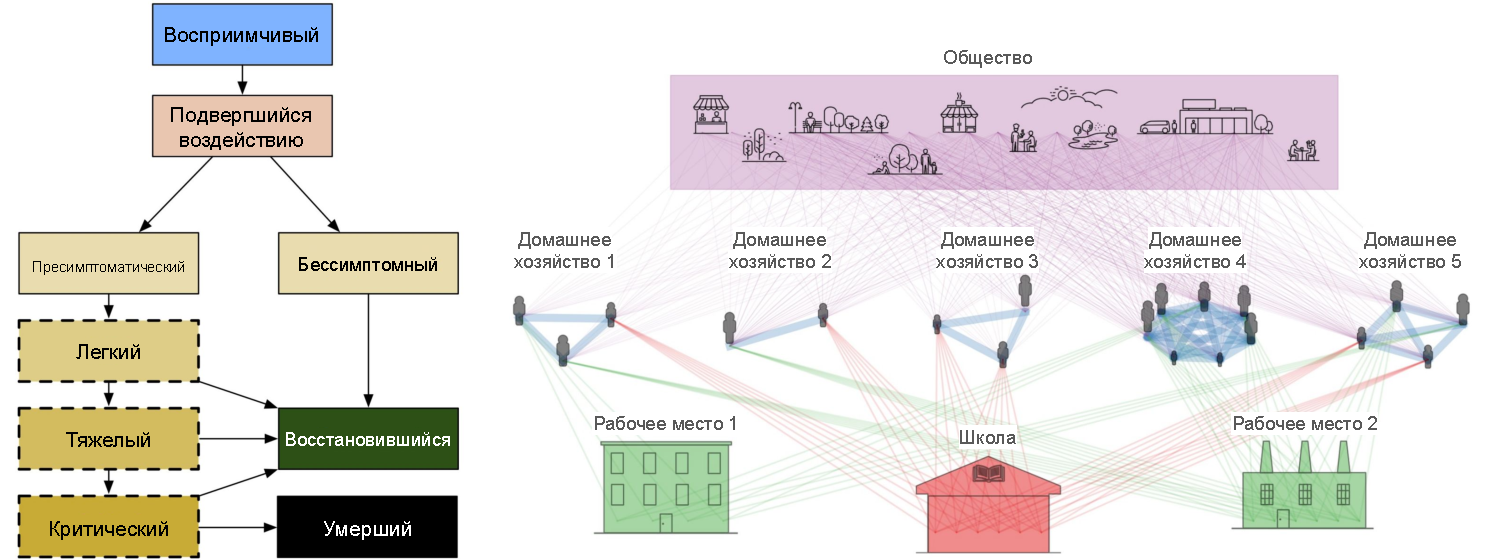
\includegraphics[width=\linewidth]{images/covasim.pdf}
    \caption{Структура модели развития инфекции (слева) и иллюстрация сети контактов в \gls{covasim}. Источник: \cite{kerr2021covasim}.}
\end{figure}

В зависимости от объемов имеющихся демографических данных для запуска \gls{covasim} можно использовать 3 способа генерации синтетической популяции: случайные сети, алгоритм \texttt{SynthPops} и гибридные сети.

В отсутствие данных применяются случайные сети: всем агентам из Пуассоновского распределения определяются числа контактов, после чего в соответствии с этими значениями формируются произвольные связи между людьми.

\texttt{SynthPops} применяется при наличии информации о вероятностях взаимодействий между возрастными группами в домохозяйствах, школах, на рабочих местах, на улице; распределении численностей людей в школах; возрастной структуре школьников; отношении числа преподавателей к числу школьников; распределении численностей рабочих мест и числах трудоустроенных людей разных возрастов; распределении размеров домохозяйств, возрастов и полов членов семей. 

При формировании связей в домохозяйствах \texttt{SynthPops} сначала выбирает размеры семей из их распределения, после чего за каждой семьей закрепляет главу семейства. Остальные члены домохозяйств набираются в соответствии с вероятностями контактов в семьях и распределением возрастов в них.

Контакты между учениками в школах формируются аналогично, собирая агентов по семьям (дети из одних домохозяйств в одних школах), после чего выбираются агенты-работники учебного заведения и в зависимости от размера школы либо создаются контакты между всеми школьниками и работниками, либо каждому работнику определяется число связей с учениками, которые затем формируются.

Связи на рабочих местах формируются аналогично из агентов случайных домохозяйств.

Для создания гибридной сети необходимы данные о распределении возрастов и размеров семей, однако они уже загружены в \gls{covasim} для каждой страны. Гибридный подход не учитывает распределение возрастов в домохозяйствах, все дети (все агенты от 6 до 22 лет) объединяются в школы, взрослые (агенты возрастом между 22 и 65) в рабочие места с предопределенными для них числами контактов в этих слоях из распределения Пуассона с различными средними значениями. Это позволяет воссоздать некоторую популяционную гетерогенность в случае недостатка демографических данных.



\subsection{Дисперсионный анализ чувствительности математических моделей}

В данной работе анализ чувствительности модели проводился с помощью дисперсионных методов в связи с ее стохастичностью и их информативностью. Недостатком являются большие вычислительные затраты. Такие методы никак не зависят от природы модели и позволяют оценить влияние изменений любых комбинаций параметров \cite{saltelli2008global}.

Пусть задана квадратично интегрируемая функция $f$ на $\Omega^k$, единичном k-мерном гиперкубе,
\begin{displaymath}
\Omega^k=(X|0\leq x_i \leq 1;i=1,\ldots ,k),
\end{displaymath}
Илья Меерович Соболь предложил раскладывать эту функцию в сумму по возрастающим размерностям:
\begin{displaymath}
f=f_0+\sum\limits_i f_i + \sum\limits_i \sum\limits_{j>i} f_{ij}+\ldots+f_{12\ldots k},
\end{displaymath}
где каждое слагаемое также является квадратично интегрируемым на области определения и является функцией лишь параметров, индексы которых указаны в его индексе, то есть $f_i=f_i(X_i)$, $f_{ij}=f_{ij}(X_i,X_j)$ и так далее. Соболь показал, что слагаемые суммы можно последовательно вычислить из результатов расчетов модели $Y$ как
\begin{align*}
&f_0=E(Y) \\
&f_i=E(Y|X_i)-E(Y) \\
&f_{ij} = E(Y|X_i,X_j)-f_i-f_j-E(Y)
\end{align*}

Оказывается, что дисперсия условного матожидания может быть использована как показатель чувствительности. Дисперсии слагаемых в приведенном выше разложении и есть искомые меры. К примеру, $V(f_i(X_i))$ есть $V[E(Y|X_i)]$, поэтому индекс чувствительности первого порядка вводится как
\begin{displaymath}
S_i=\frac{V[E(Y|X_i)]}{V(Y)}.
\end{displaymath}

Индекс первого порядка представляет собой основной вклад варьирования каждого параметра в дисперсию модели и был описан разными учеными как мера важности \cite{hora1986comparison, ishigami1990importance, iman1990robust, saltelli1993sensitivity, homma1996importance}.

Тогда же Соболь предложил эквивалентное определение \cite{sobol1996freezing}, основанное на корреляции между результатами модели $Y$ и условным матожиданием $E(Y|X_i)$
\begin{displaymath}
S_i=\text{Corr}(Y,E(Y|X_i)).
\end{displaymath}

С учетом того, что $V_i=V(f_i(X_i))=V[E(Y|X_i)]$ выражение
\begin{displaymath}
V_{ij}=V(f_{ij}(X_i,X_j))=V(E(Y|X_i,X_j))-V(E(Y|X_i))-V(E(Y|X_j))
\end{displaymath}
позволяет оценить эффект совместного варьирования $(X_i,X_j)$ на результат $Y$, который называют индексом чувствительности второго порядка $S_{ij}$ \cite{box1978statistics}. Аналогичные формулы могут быть выписаны для индексов высших порядков, основываясь на analysis of variance high-dimensional model representation (анализ дисперсии по многомерному представлению) (ANOVA-HDMR) разложении
\begin{displaymath}
V(Y)=\sum\limits_i V_i + \sum\limits_i \sum\limits_{j>i} V_{ij}+\ldots +V_{123\ldots k}.
\end{displaymath}
Деля обе части равенства на $V(Y)$, получаем
\begin{displaymath}
\sum\limits_i S_i + \sum\limits_i \sum\limits_{j>i} S_{ij}+\ldots +S_{123\ldots k}=1.
\end{displaymath}

Также возможно оценить вклад варьирования параметра и всех связанных с ним взаимодействий вычислением полного индекса Соболя
\begin{displaymath}
S_{T_i}=\frac{E[V(Y|\bm{X}_{\sim i})]}{V(Y)}=1-\frac{V[E(Y|\bm{X}_{\sim i})]}{V(Y)},
\end{displaymath}
где $\bm{X}_{\sim i}$ --- множество всех параметров, кроме $X_i$.
\subsection{Гравитационные модели транспортных потоков}
В отсутствие достаточных объемов данных о перемещениях людей величины транспортных потоков оценивают с помощью гравитационных моделей. Такую модель исследовали Бушар и Паерс (1965) \cite{bouchard1965use}. На основе данных опросов разных лет о перемещениях в Вашингтоне авторы проверили точность гравитационной модели при прогнозировании распределений городских поездок. В качестве метрики качества предсказания авторы использовали среднеквадратичное отклонение оцененных чисел поездок между парами зон Вашингтона от фактических из результатов опросов, деленное на среднее число поездок. Модель представляется уравнением

\begin{displaymath}
T_{i-j}=\frac{P_iA_jF_{(t_{i-j})}K_{(i-j)}}{\sum\limits_{x=1}^nA_xF_{(t_{i-x})}K_{(i-x)}},
\end{displaymath}
где \\ $P_i$ --- количество поездок из зоны $i$, \\ $A_j$ --- количество поездок в зону $j$, \\ $t_{i-j}$ --- мера пространственного разделения (сумма минимального времени перемещения из зоны $i$ в $j$ и терминального времени), \\ $F_{(t_{i-j})}$ --- эмпирический временной фактор, показывающий убывание транспортных потоков с возрастанием времени поездки, \\ $K_{(i-j)}$ --- калибровочный коэффициент.

Авторы показали, что при правильной калибровке такая модель показывает высокую точность (нормированное среднеквадратичное отклонение чисел поездок менее 15\% для крупных потоков), а факторы $F_{(t_{i-j})}$ стабильны во времени. Однако для достижения такой точности необходима стратификация поездок по их цели.



\section{Материалы и методы}
\subsection{Используемые программные пакеты}
\begin{table}[H]
\centering
\begin{tabular}{p{4cm} p{10cm}}
\toprule
\textbf{Модуль} & \textbf{Назначение} \\
\midrule
\texttt{numpy} \cite{harris2020array} & Обработка многомерных массивов \\
\texttt{pandas} \cite{reback2020pandas} & Обработка табличных баз данных \\
\texttt{matplotlib} \cite{Hunter:2007} & Визуализация данных \\
\texttt{seaborn} \cite{michael_waskom_2017_883859} & Визуализация данных (тепловые карты, ящики с усами) \\
\texttt{scipy} \cite{2020SciPy-NMeth} & Проведение статистических тестов, линейной аппроксимации, вычисление коэффициента корреляции Пирсона \\
\texttt{SALib} \cite{Iwanaga2022, Herman2017} & Вычисление последовательности Соболя и индексов Соболя \\
\bottomrule
\end{tabular}
\caption{Используемые модули \texttt{Python}.}
\end{table}
\subsection{Реализация транспортных потоков в исследуемой модели}

Все основные алгоритмы в цикле симуляции \gls{covasim}, такие как вычисление восприимчивости и трансмиссивности агентов и определение новых зараженных агентов, реализованы с помощью высокооптимизированных операций над 32-битными массивами \texttt{Numba}. Для достижения большей эффективности агенты представлены не отдельными объектами, а в виде срезов набора массивов состояний.

На каждом шаге симуляции в каждом городе выбираются случайные агенты-туристы, количество которых согласуется с величинами транспортных потоков. Агент-турист удаляется из сети контактов своего населенного пункта и внедряется в город прибытия. Там он вступает в фиксированное число случайных контактов. По завершении периода поездки производится обратная операция. Перемещениям не подвержены агенты в тяжелом или критическом состоянии. Если они оказываются в списке туристов, то не покидают свой город. Если же они оказались в таком состоянии по завершении периода поездки, они возвращаются в родной город только при выздоровлении.

Для реализации транспортных потоков мы расширили набор массивов состояний 4 аттрибутами агентов, что изображено на Рис. \ref{pic:array}:
\begin{enumerate}
\item \texttt{trueId} хранит идентификаторы, которые агенты имели, находясь в родном городе, чтобы восстановить их при возвращении агентов;
\item \texttt{inCity} хранит булевые значения нахождения агентов в городе;
\item \texttt{restInAnotherCityDays} хранит число оставшихся дней нахождения агентов в другом городе;
\item \texttt{ownCity} хранит идентификаторы родного города агентов.
\end{enumerate}

\begin{figure}[]
    \centering
    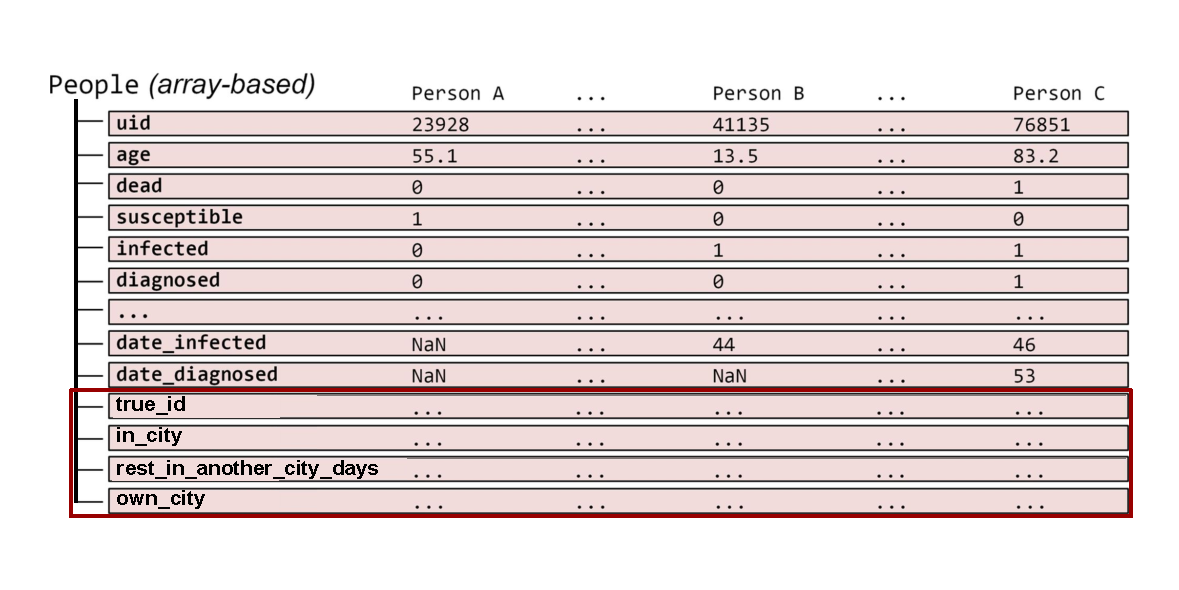
\includegraphics[width=0.8\linewidth]{images/arrays.pdf}
    \caption{Матричный подход представления агентов в \gls{covasim} с добавленными нами аттрибутами. Источник: \cite{kerr2021covasim}.}
    \label{pic:array}
\end{figure}

Возможность помещения агентов-туристов в города обеспечивается выделением в них агентов-<<пустышек>>, не участвующих во взаимодействиях, так как отмечены как отсутствующие в городе (\(\texttt{inCity} = \texttt{False}\)). К синтетической популяции они подключены посредством слоя контактов \texttt{touristLayer} с основными параметрами из \texttt{randomLayer}. По приезде в город агенты-туристы вместе со всеми своими свойствами замещают в городе прибытия агентов-<<пустышек>> и включаются в социальные взаимодействия. Такой подход позволяет не изменять размеры массивов во время вычислений.

Для произведения параллельных вычислений используется модуль \texttt{multiproces\-sing} языка \texttt{Pyt\-hon}, с помощью которого создаются процессы, каждый из которых параллельно симулирует происходящее в одном городе, периодически синхронизируясь и обмениваясь информацией о перемещающихся агентов. Именно \texttt{multiprocessing}, а не \texttt{multithreading} применяется нами, так как создает отдельные процессы со своими \gls{gil}. Это позволяет эффективно работать на нескольких ядрах центрального процессора, а значит, и масштабировать вычисления при работе на кластерах. \texttt{Multithreading} же используют один процесс, в рамках которого выделяются потоки, из-за чего имеют один \gls{gil} на все потоки и истинный параллелизм оказывается невозможен --- такой подход обычно применяют, если задачи не являются чисто вычислительными и потоки много времени проводят в режиме ожидания внешних операций.

В текущей версии модели у туристических потоков можно настроить следующие параметры:

\begin{enumerate}
\item \texttt{adjacencyMatrix}: матрица контактов городов, показывающая величины транспортных потоков из одного города в другой в долях населения города отправления;
\item \texttt{timeRelax}:  средняя длительность нахождения агента в другом городе, по умолчанию 7;
\item \texttt{interventionData}: информация об ограничениях на транспортные потоки --- словарь, содержащий информацию о том, какой конкретно транспортный поток ограничивается, в какой день вступают в силу эти ограничения, какова их длительность и во сколько раз уменьшаются потоки из-за введения ограничений;
\item \texttt{contactCount}: среднее число контактов у агента-туриста с местными жителями, по умолчанию 40;
\item \texttt{beta}: множитель вероятности передачи инфекции в туристическом слое, по умолчанию 0.3.
\end{enumerate}

При запуске симуляции в режиме нескольких городов схема вычислений:

\begin{enumerate}
	\item Инициализация;
	\item Барьер синхронизации процессов;
	\item Цикл симуляции:
	\begin{enumerate}
		\item Обмен агентами-туристами между процессами (функции \texttt{AddBack} и \texttt{AddTourists});
		\item Основной шаг симуляции;
		\item Барьер синхронизации процессов;
		\item Определение отправляемых агентов-туристов (функции \texttt{ExtractBack} и \texttt{Extract\-Tourists});
		\item Барьер синхронизации процессов.
	\end{enumerate}
	\item Обработка и визуализация результатов.
\end{enumerate}

\subsubsection{Инициализация}
На этапе инициализации для каждого города определяется выделяемое число мест под туристов как доля численности населения города равная
\begin{displaymath}
\max\left(0.1,\sum\limits_j \frac{2\cdot\texttt{timeRelax}}{\texttt{maxMultCoef}\cdot\texttt{adjacencyMatrix}[i,j]}\right),
\end{displaymath}
другими словами, под туристов выделяется число мест больше или равное удвоенному математическому ожиданию их количества при значении \texttt{maxMultCoef} по умолчанию равном единице.

Затем эти агенты добавляются в города как отсутствующие (\(\texttt{inCity}=\texttt{False}\)) и внедряются в социальные взаимодействия с помощью \texttt{touristLayer} в соответствии с заданными параметрами. 

После инициализации модель входит в главный цикл симуляции.

\subsubsection{Функция внедрения перемещаемых агентов в город назначения}

Данная функция передает агентам в городе назначения под индексами \texttt{inds} все атрибуты агентов-туристов \texttt{rest}, кроме идентификатора \texttt{uid}, после чего обозначает их присутствие в городе (\(people.inCity[inds] \gets True\)). Этот алгоритм приведен в Псевдокоде \ref{alg:updatepeoplebyrest}.

\begin{algorithm}[H]
\caption{Функция внедрения перемещаемых агентов в город назначения}
\label{alg:updatepeoplebyrest}
\begin{algorithmic}[1]
\Function{UpdatePeopleByRest}{$people, rest, inds$}
	\For{\(each\) \(arrayMember\) \textbf{in} \(people.arrayMembers\)}
		\If{\(arrayMember \neq uid\)}
			\State \(people[arrayMember][inds] \gets rest[arrayMember]\)
		\EndIf
	\EndFor
	\State \(people.inCity[inds] \gets True\)
\EndFunction
\end{algorithmic}
\end{algorithm}

\subsubsection{Функция возвращения агентов в родной город}

Данная функция возвращает агентов \texttt{backPeople} в соответствии с их родным идентификатором \texttt{backPeople.trueUid} с помощью функции \texttt{UpdatePeopleByRest}. 


\subsubsection{Функция размещения агентов-туристов в городе назначения}

Данная функция определяет доступные под размещение туристов идентификаторы в городе назначения, выбирает из них необходимое количество соответствующее числу приезжающих туристов, если им хватает мест, или все оставшиеся места в противном случае. Затем на места по выбранным идентификаторам размещаются агенты с помощью функции \texttt{UpdatePeopleByRest}. Этот алгоритм приведен в Псевдокоде \ref{alg:addtourists}.

\begin{algorithm}[H]
\caption{Функция размещения агентов-туристов в городе назначения}
\label{alg:addtourists}
\begin{algorithmic}[1]
\Function{AddTourists}{$people, tourists$}
	\State \(allTouristsInds\) \(\gets\) \(people.uid[(people.uid \geqslant people.popSize)\) \(*\) \((\)\textbf{not} \(people.inCity)]\)
	\State \(freeTouristsInds\) \(\gets\) \(allTouristsInds[:tourists.popSize]\)
	\State \(updatePeopleByRest(people.tourists,freeTouristsInds)\)
\EndFunction
\end{algorithmic}
\end{algorithm}

\subsubsection{Функция выбора уезжающих агентов и их извлечения из города}
Данная функция в соответствии с долей ежедневно уезжающих из города туристов \texttt{outflowRatio} задает их количество из распределения Пуассона. Затем это число идентификаторов агентов выбирается среди местных жителей (\texttt{people.uid} < \texttt{people.pop\-Size}), находящихся в городе (\texttt{people.inCity == True}). Этот список разбивается на списки по городам назначения из известных соотношений транспортных потоков \texttt{outflow\-RatioToCitiesPercent}. Для каждого города назначения \texttt{cityInd} из списка туристов удаляются тяжелые, критические, мертвые. Оставшимся назначается длительность пребывания в другом городе \texttt{people.restInAnotherCityDays} либо тождественно равная 1 для всех при моделировании потоков рабочих, либо из распределения Пуассона без 0 в противном случае. Затем все отъезжающие агенты из списка \texttt{touristPeople} извлекаются из города отправления и сохраняются в виде списка пар (\texttt{cityInd}, \texttt{touristPeople}). Этот алгоритм приведен в Псевдокоде \ref{alg:extracttourists}.

\begin{algorithm}[H]
\caption{Функция выбора уезжающих агентов и их извлечения из города}
\label{alg:extracttourists}
\begin{algorithmic}[1]
\Function{ExtractTourists}{people}
	\State \( allPeopleLeftCityCount \gets Poisson(people.popSize * outflowRatio) \)
	\State \( inCityRestrictionInds \gets people.uid[people.inCity * (people.uid < people.popSize)]\)
	\State \( allPeopleLeftCityInds \gets \) \(random\) \(selection\) \(of\) \(allPeopleLeftCityCount\) \(indices\) \(from\) \(0\) \(to\) \(len(inCityRestrictionInds)\)
	\State \( peopleLeftCityToCityInds \) \(\gets\) \(split(allPeopleLeftCityInds,outflowRatioToCities\-Percent) \)
	\State \( listTouristPeople \gets\) \(empty\) \(list \)
	\For{\( cityInd \gets 0\) \textbf{to} \( citiesCount - 1 \)}
		\If{\( cityInd = ownInd \)}
			\State \textbf{continue}
		\EndIf
		\State \( touristPeopleIndsInCity \gets peopleLeftCityToCityInds[cityInd] \)
		\State \( touristPeopleInds \gets inCityRestrictionInds[touristPeopleIndsInCity] \)
		\State \( touristPeopleIndsFiltered\) \( \gets \) \( select \) \( indices \) \( from \) \( touristPeopleInds \) \( where \) \textbf{not} \( (people.severe \) \textbf{or} \( people.critical \) \textbf{or} \( people.dead) \)
		\State \( touristPeople \gets \) \(select\) \(people\) \(with\) \(indices\) \(touristPeopleIndsFiltered \)
		\If{\(lambda == 0\)}
			\State \( restInAnotherCityDays \gets Ones(touristPeople.popSize) \)
		\Else
			\State \( restInAnotherCityDays \gets ZeroTruncatedPoisson(lambda, touristPeople.pop\-Size) \)
		\EndIf
		\State \( append(cityInd, touristPeople) \) \(to\) \(listTouristPeople \)
	\EndFor
	\State \(remove\) \(people\) \(with\) \(indices\) \(allPeopleLeftCityInds\) \(from\) \(people \)
	\State \Return \( listTouristPeople \)	
\EndFunction	
\end{algorithmic}
\end{algorithm}


\subsubsection{Функция выбора возвращаемых агентов и их извлечения из города}

Данная функция определяет индексы агентов, чей родной город соответствует индексу в цикле (\texttt{people.ownCity == cityInd}), время поездки которых кончилось (\texttt{people.restInAnotherCityDays == 0}) и которые на текущий шаг симуляции не являются тяжелыми, критическими или мертвыми. После этого агенты с этими индексами \texttt{backPeople} извлекаются из города их нахождения и добавляются в список возвращаемых как пара (\texttt{cityInd}, \texttt{backPeople}). Этот алгоритм приведен в Псевдокоде \ref{alg:extractback}.

\begin{algorithm}[H]
\caption{Функция выбора возвращаемых агентов и их извлечения из города}
\label{alg:extractback}
\begin{algorithmic}[1]
\Function{ExtractBack}{people}
	\State \(listBackPeople \gets empty \) \(list\)
	\For{\(cityInd \gets 0\) \textbf{to} \(citiesCount - 1\)}
		\If{\(cityInd = ownInd\)}
			\State \textbf{continue}
		\EndIf
		\State \(shouldBackCityInds\) \(\gets\) \(find\) \(people\) \(who\) \(should\) \(return\) \(to\) \(their\) \(own\) \(city\) \textbf{and} \(who\) \(is\) \textbf{not} \( (people.severe \) \textbf{or} \( people.critical \) \textbf{or} \( people.dead) \)
		\State \(backPeople\) \(\gets\) \(select\) \(people\) \(with\) \(indices\) \(shouldBackCityInds\)
		\State \(remove\) \(people\) \(with\) \(indices\) \(shouldBackCityInds\) \(from\) \(people\)
		\State \(append(cityInd, backPeople)\) \(to\) \(listBackPeople\)
	\EndFor
	\State \Return \(listBackPeople\)
\EndFunction 
\end{algorithmic}
\end{algorithm}




%\subsubsection{Отладка реализации транспортных потоков}


%При выполнении данной работы был исправлен ряд неточностей предыдущей версии модели:

%\begin{enumerate}
%\item Был введен запрет на перемещение между городами агентов в тяжелом и критическом состоянии и мертвых агентов.
%\item Ранее при создании списка отправляемых из города туристов не проводилась проверка их присутствия в городе, в связи с чем могло происходить дублирование агента как туриста.
%\item Ранее на каждом шаге симуляции оставшаяся длительность отпуска агента снижалась на единицу, если она больше или равна 0, что приводило к тому, что она могла стать равной -1 при начальной у агента 0.
%\item Ранее длительность отпуска определялась из Пуассоновского распределения, а значит часть агентов получала длительность отпуска равную 0 (причем чем меньше задаваемая средняя длительность отпуска, тем чаще это происходило) и вкупе с предыдущей уязвимостью эти агенты перемещались в другие города, их длительность отпуска становилась -1, и они уже никогда не покидали этот город. Теперь длительность отпуска определяется из Пуассоновского распределения без 0, а параметр распределения подсчитывается так, чтобы оценка его матожидания соответствовала задаваемому параметру.
%\end{enumerate}

\subsection{Вычисление индексов Соболя}
Вычисление индексов Соболя производилось с помощью модуля \texttt{SALib} \cite{Iwanaga2022, Herman2017} по следующему алгоритму \cite{saltelli2008global}:
\begin{itemize}
\item Создавалась матрица случайных значений параметров $k$ размера $(N,2k)$, определяющая матрицы $A$ и $B$. Параметры выбирались, используя последовательности псевдослучайных чисел для более равномерного заполнения пространства параметров \cite{sobol1967distribution, sobol1976uniformly} (этот факт продемонстрирован на Рис. \ref{pic_sobol})
\begin{displaymath}
A=\begin{bmatrix}
x_1^{(1)} & x_2^{(1)} & \ldots & x_i^{(1)} & \ldots & x_k^{(1)} \\
x_1^{(2)} & x_2^{(2)} & \ldots & x_i^{(2)} & \ldots & x_k^{(2)} \\
\ldots & \ldots & \ldots & \ldots & \ldots & \ldots \\
x_1^{(N-1)} & x_2^{(N-1)} & \ldots & x_i^{(N-1)} & \ldots & x_k^{(N-1)} \\
x_1^{(N)} & x_2^{(N)} & \ldots & x_i^{(N)} & \ldots & x_k^{(N)} \\
\end{bmatrix},
\end{displaymath}
\begin{displaymath}
B=\begin{bmatrix}
x_{k+1}^{(1)} & x_{k+2}^{(1)} & \ldots & x_{k+i}^{(1)} & \ldots & x_{2k}^{(1)} \\
x_{k+1}^{(2)} & x_{k+2}^{(2)} & \ldots & x_{k+i}^{(2)} & \ldots & x_{2k}^{(2)} \\
\ldots & \ldots & \ldots & \ldots & \ldots & \ldots \\
x_{k+1}^{(N-1)} & x_{k+2}^{(N-1)} & \ldots & x_{k+i}^{(N-1)} & \ldots & x_{2k}^{(N-1)} \\
x_{k+1}^{(N)} & x_{k+2}^{(N)} & \ldots & x_{k+i}^{(N)} & \ldots & x_{2k}^{(N)} \\
\end{bmatrix}.
\end{displaymath}

\begin{figure}[H]
    \centering
    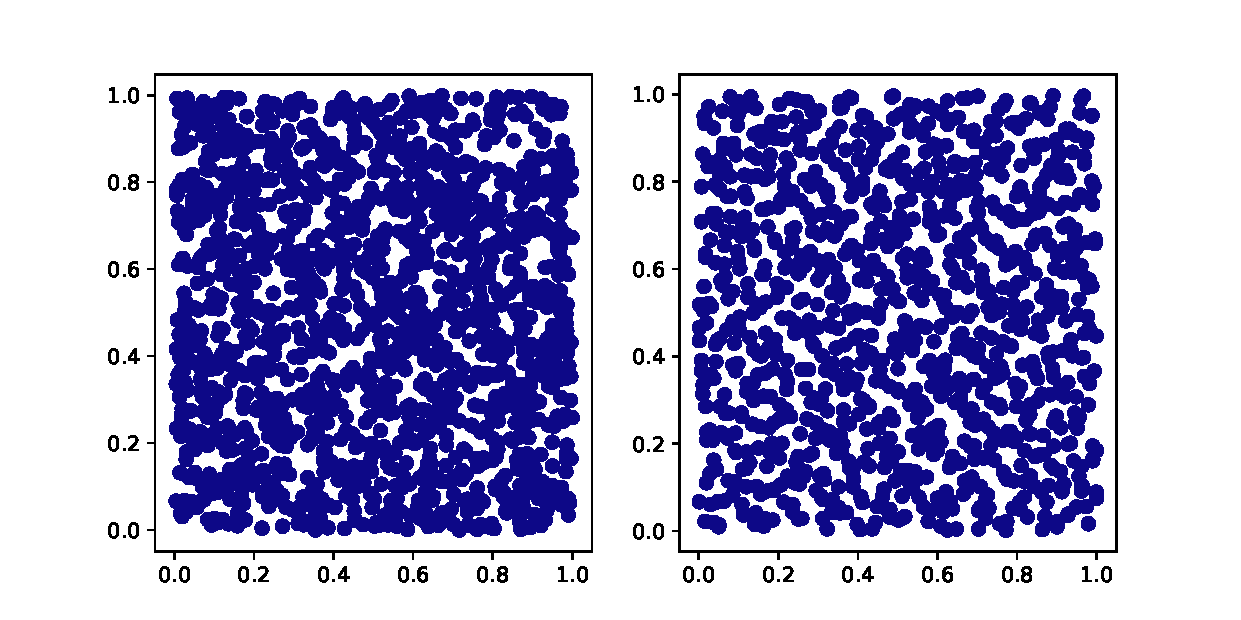
\includegraphics[width=\linewidth]{images/sampling.pdf}
    \caption{Наборы точек из двумерного пространства, взятые из равномерного случайного распределения (слева) и последовательности псевдослучайных чисел Соболя (справа).}
    \label{pic_sobol}
\end{figure}

\item Создавалась матрица $C_i$ так, что ее столбцы с индексами, кроме $i$, были равны соответствующим столбцам матрицы $B$, а столбец с индексом $i$ был равен столбцу матрицы $A$ с тем же индексом:
\begin{displaymath}
C_i=\begin{bmatrix}
x_{k+1}^{(1)} & x_{k+2}^{(1)} & \ldots & x_i^{(1)} & \ldots & x_{2k}^{(1)} \\
x_{k+1}^{(2)} & x_{k+2}^{(2)} & \ldots & x_i^{(2)} & \ldots & x_{2k}^{(2)} \\
\ldots & \ldots & \ldots & \ldots & \ldots & \ldots \\
x_{k+1}^{(N-1)} & x_{k+2}^{(N-1)} & \ldots & x_i^{(N-1)} & \ldots & x_{2k}^{(N-1)} \\
x_{k+1}^{(N)} & x_{k+2}^{(N)} & \ldots & x_i^{(N)} & \ldots & x_{2k}^{(N)} \\
\end{bmatrix}.
\end{displaymath}
\item Вычислялся вывод модели при всех наборах параметров из матриц $A$, $B$, $C_i$, то есть получались три вектора длины $N$:
\begin{displaymath}
y_A=f(A)\qquad y_B=f(B) \qquad y_{C_i}=f(C_i).
\end{displaymath} 
\item Вычислялся индекс Соболя первого порядка
\begin{displaymath}
S_i=\frac{V[E(Y|X_i)]}{V(Y)}=\frac{y_A\cdot y_{C_i}-f_0^2}{y_A\cdot y_A -f_0^2}=\frac{(1/N)\sum_{j=1}^N y_A^{(j)}y_{C_i}^{(j)} - f_0^2}{(1/N)\sum_{j=1}^N (y_A^{(j)})^2 - f_0^2},
\end{displaymath}
где
\begin{displaymath}
f_0^2=\left(\frac{1}{N}\sum\limits_{j=1}^N y_A^{(j)}\right)^2.
\end{displaymath}

Аналогично полный индекс Соболя
\begin{displaymath}
S_{T_i}=1-\frac{V[E(Y|\bm{X}_{\sim i})]}{V(Y)}=1-\frac{y_B\cdot y_{C_i}-f_0^2}{y_A\cdot y_A -f_0^2}=1-\frac{(1/N)\sum_{j=1}^N y_B^{(j)}y_{C_i}^{(j)} - f_0^2}{(1/N)\sum_{j=1}^N (y_A^{(j)})^2 - f_0^2}.
\end{displaymath}
\end{itemize}

Преимуществом такого подхода является тот факт, что для вычисления индексов по $k$ параметрам требуется только $N(k+2)$ запусков симуляции в отличие от полного перебора $N^2$ точек пространства параметров. Метод позволяет вычислить только полные индексы и индексы первого порядка, но они являются самыми информативными, поэтому мы ограничились ими в данной работе \cite{saltelli2008global}.

\subsection{Доступ к исходным материалам}
Материалы проекта, в том числе исходные коды для проведения экспериментов и обработки их результатов, доступны в репозитории GitHub: \url{https://github.com/KonstantinKlochkovv/bachelor-thesis}.

\newpage
\section{Результаты}

\subsection{Модель связи двух городов с одинаковой численностью агентов}
Данный эксперимент был поставлен на модели из двух идентичных городов с населением по 100 тысяч человек, транспортные потоки между которыми были равны. Схематичное представление транспортной модели представлено на Рис. \ref{pic:basicflows}. При различных величинах этих потоков (в долях населения в день) и трансмиссивности инфекции (в долях трансмиссивности уханьского варианта \gls{sars}) были запущены по 150 симуляций эпидемии при начале в одном из городов. Среднее время пребывания туриста в городе назначения --- 7 дней, число контактов --- 40, множитель трансмиссивности для туристов --- 0.3 (как у случайных контактов в \gls{covasim}). Перед дальнейшей обработкой полученных эпидемиологических кривых были удалены выбросы --- симуляции, в которых эпидемия не началась вовсе и в которых она не перешла во второй город. 

\begin{figure}[H]
    \centering
    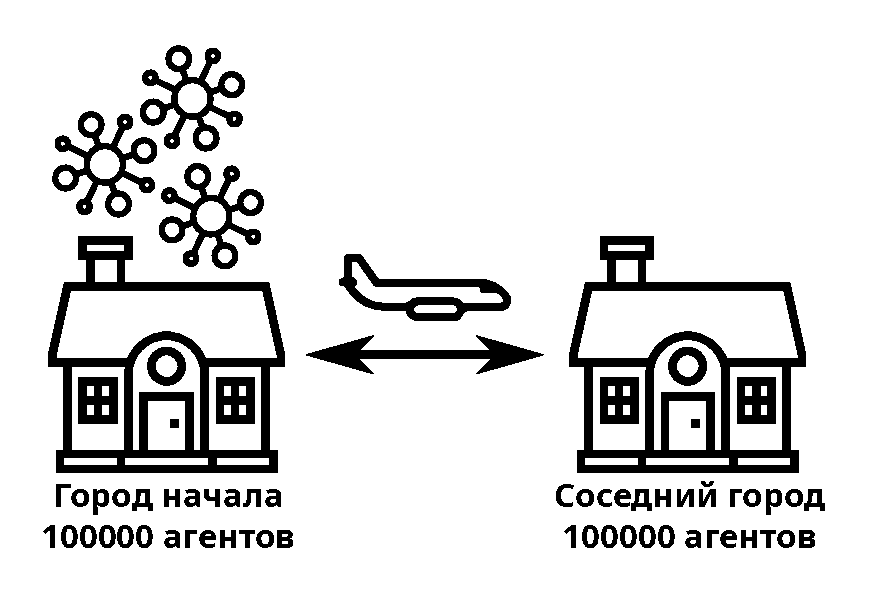
\includegraphics[width=0.5\linewidth]{images/basicflows.pdf}
    \caption{Схематичное представление простейшей исследуемой модели транспортных потоков.}
    \label{pic:basicflows}
\end{figure}


В результате оказалось, что сдвиг эпидемиологической кривой эпидемии во втором городе относительно первого оказался монотонно убывающей функцией трансмиссивности и транспортного потока, как и разброс результатов, что продемонстрировано на Рис. \ref{pic:flows_epids_lines} -- \ref{pic:flows_lines}.

На Рис. \ref{pic:flows_heatmap_conference} приведены тепловые карты среднего сдвига дня пика эпидемии (слева) и t-статистики при сравнении дней пика в рассматриваемых городах (справа). Наблюдается, что в отличие от среднего сдвига дня пика t-статистика монотонно возрастает с увеличением трансмиссивности и убывает с увеличением транспортного потока. Также следует отметить, что при пороговом уровне значимости 0.05 критическое значение t-статистики составляет $1.96$, то есть при транспортных потоках $\leqslant 0.003$ между двумя городами наблюдается статистически значимая разница между временами пиков инфицирований.

На Рис. \ref{pic:flows_lines} изображены зависимости среднего смещения (слева) и t-статистики смещения дня пика (справа) от величины транспортного потока при различных трансмиссивностях инфекции. Оказалось, что средний сдвиг дня пика является линейной функцией логарифма величины транспортного потока, причем угловой коэффициент ее наклона тем меньше по модулю, чем больше трансмиссивность (коэффициент детерминации $R^2 \in [0.983, 0.995]$). t-статистика же является немонотонной выпуклой вверх функцией транспортного потока с максимумом при величине потока $< 10^{-4}$.

\begin{figure}[H]
    \centering
    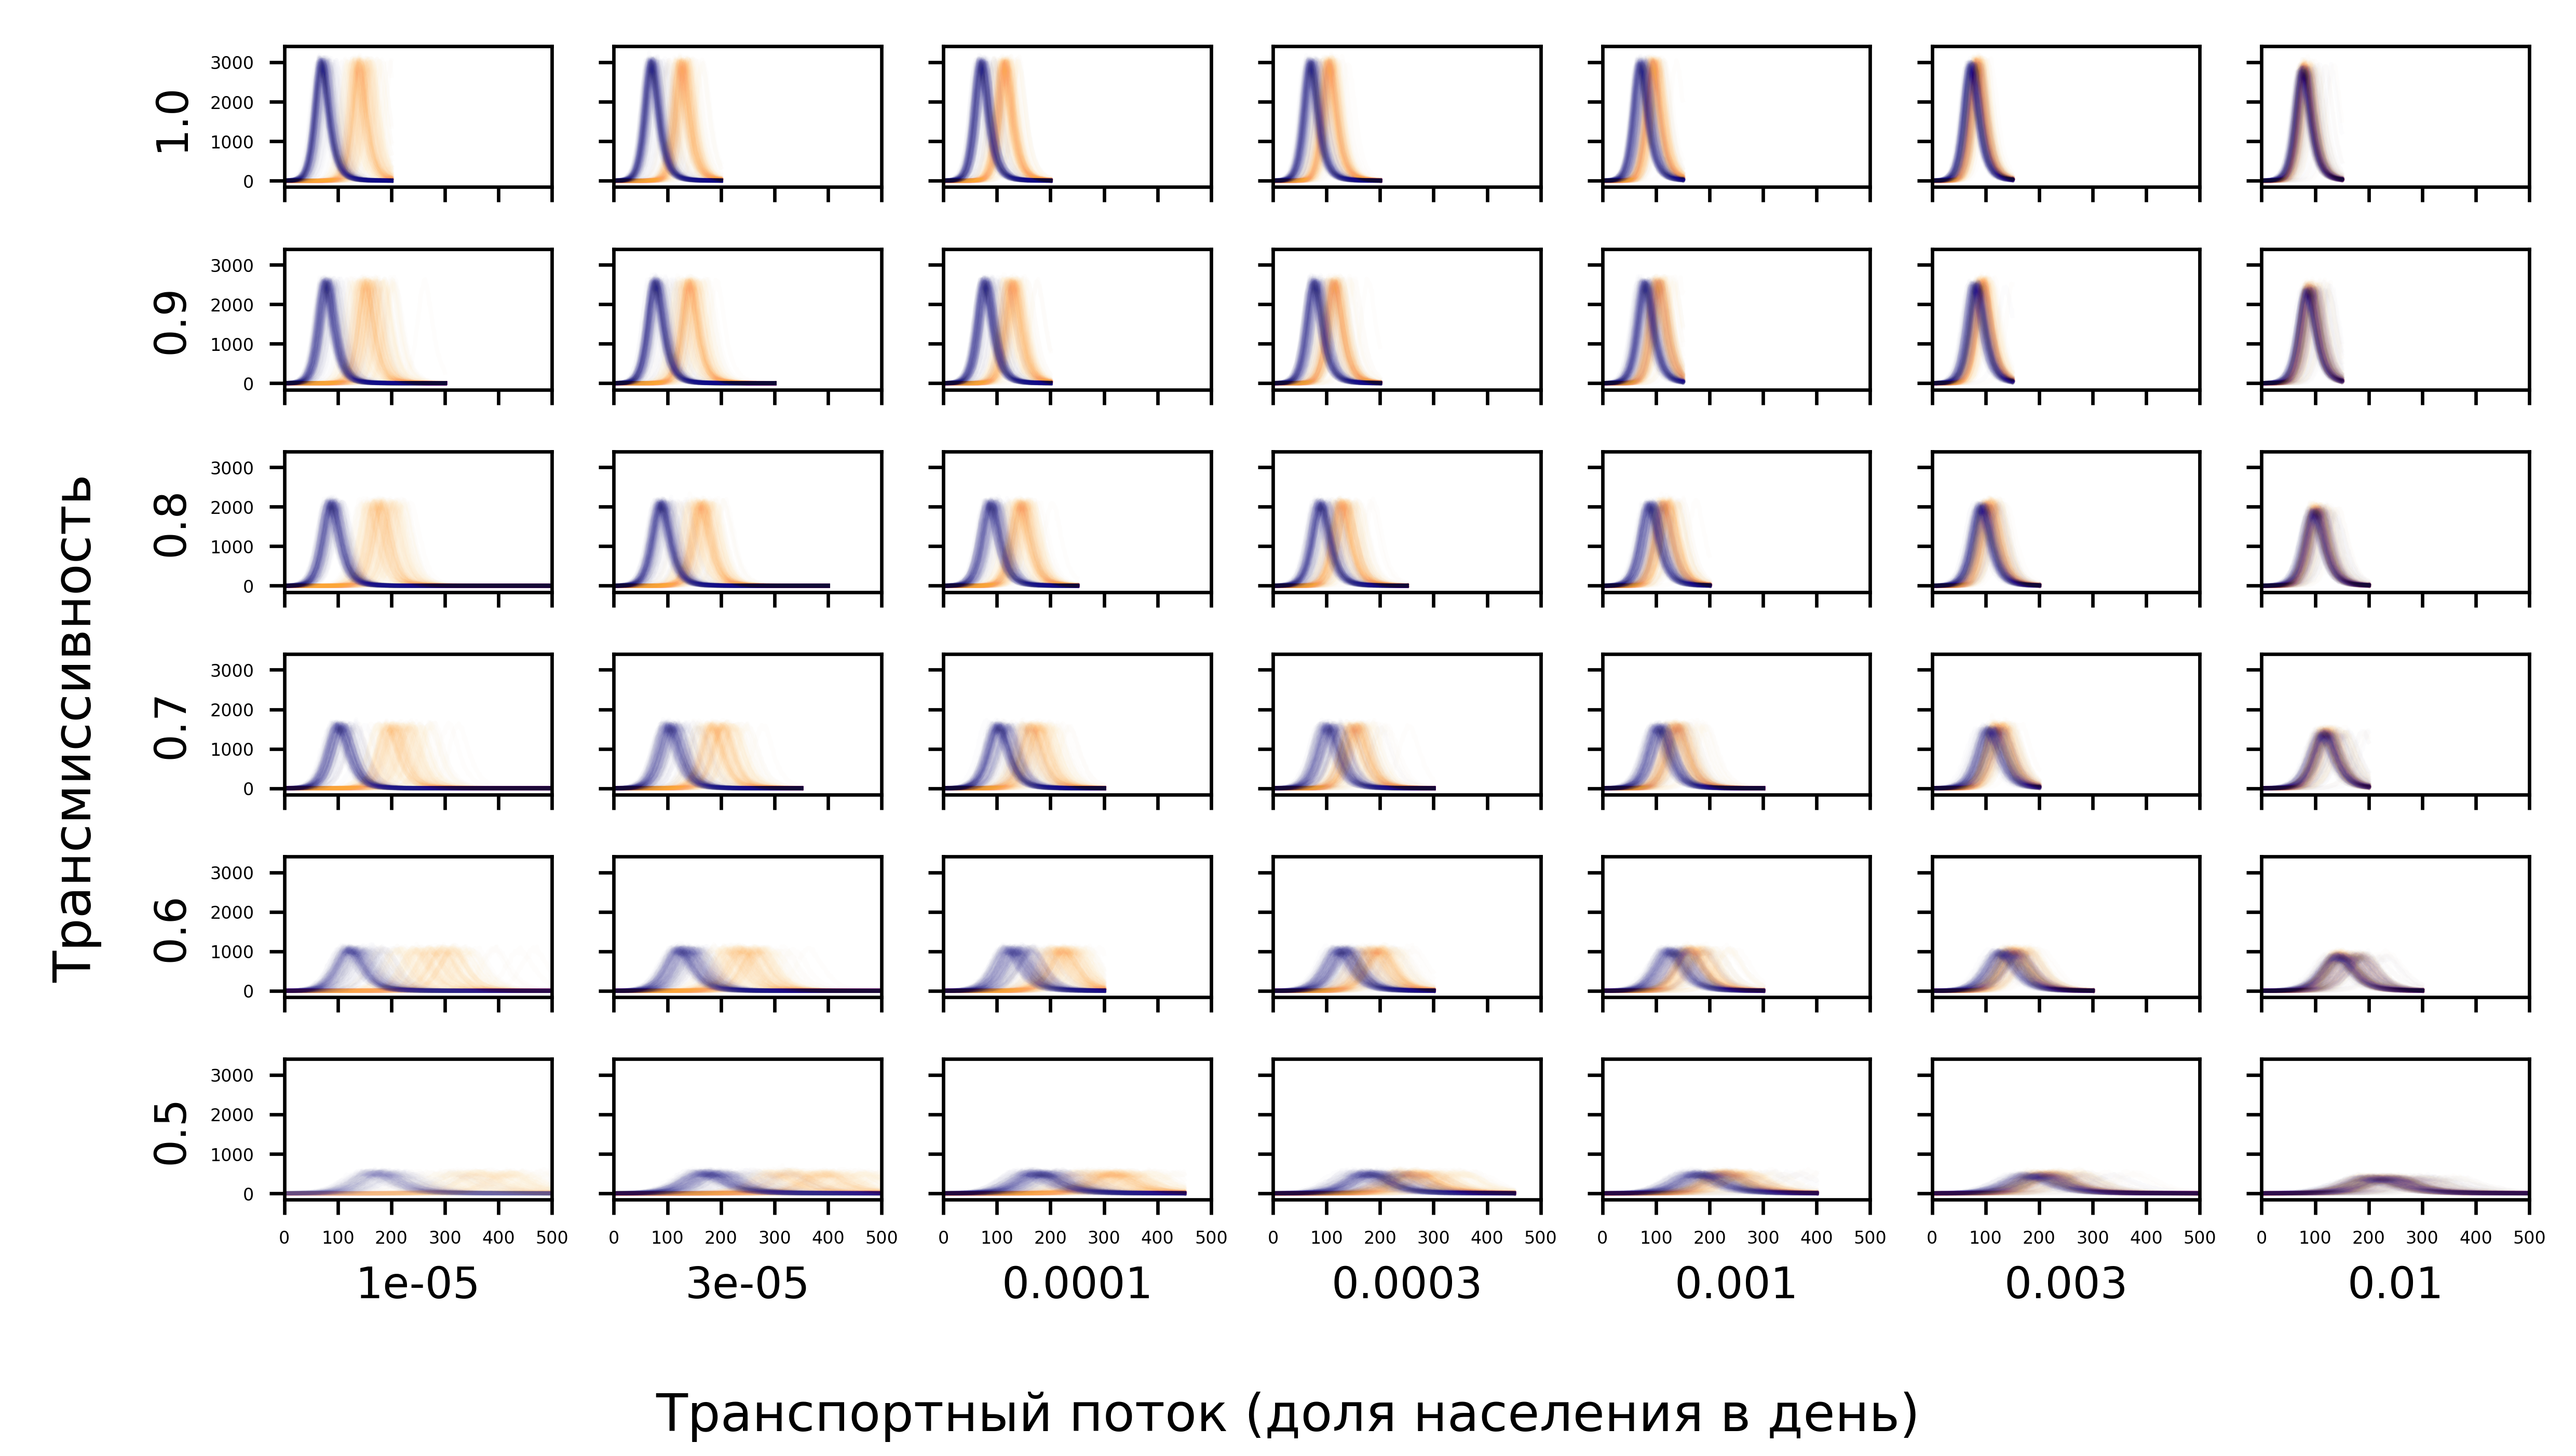
\includegraphics[width=0.95\linewidth]{images/flows_epids_lines.pdf}
    \caption{Эпидемиологические кривые по результатам моделирования двух городов при разных трансмиссивностях инфекции и пассажиропотоках (на каждом графике 150 экспериментов).}
    \label{pic:flows_epids_lines}
\end{figure}

\begin{figure}[H]
    \centering
    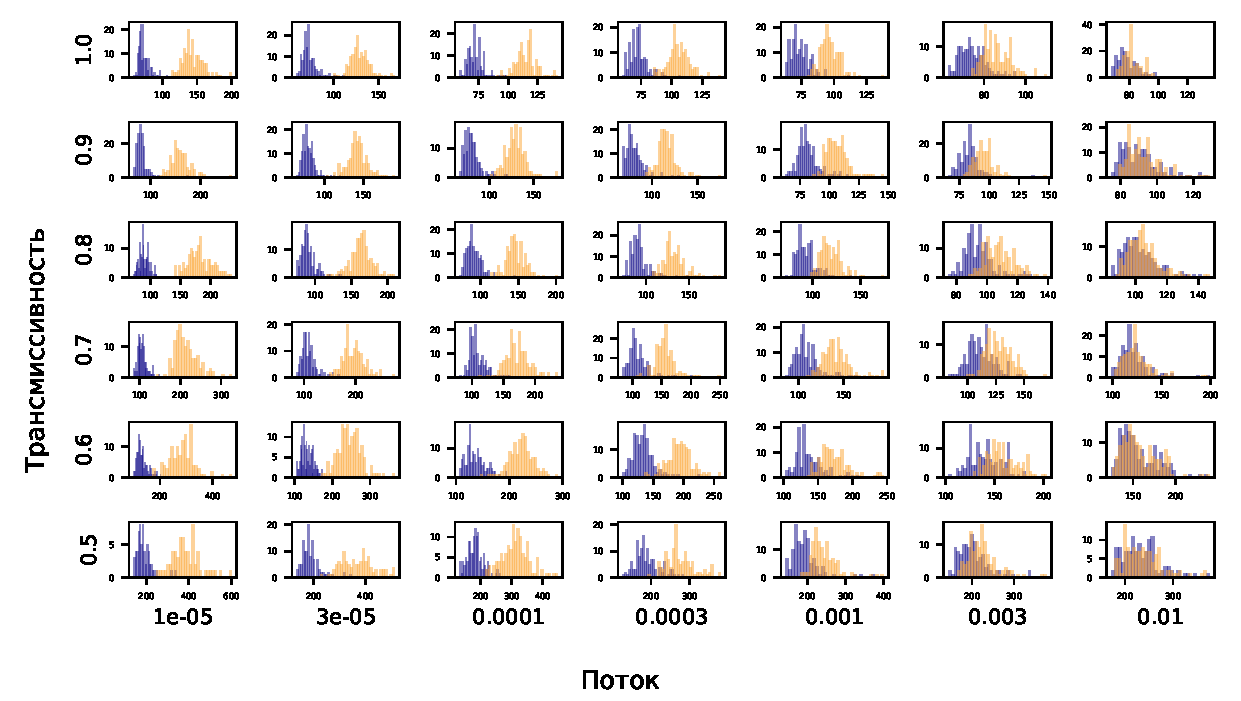
\includegraphics[width=0.95\linewidth]{images/flows_hists_day.pdf}
    \caption{Гистограммы распределения дня пика инфицирований для двух городов (синяя соответствует городу начала эпидемии, оранжевая --- второму городу).}
    \label{pic:flows_hists_day}
\end{figure}

\begin{figure}[H]
    \centering
    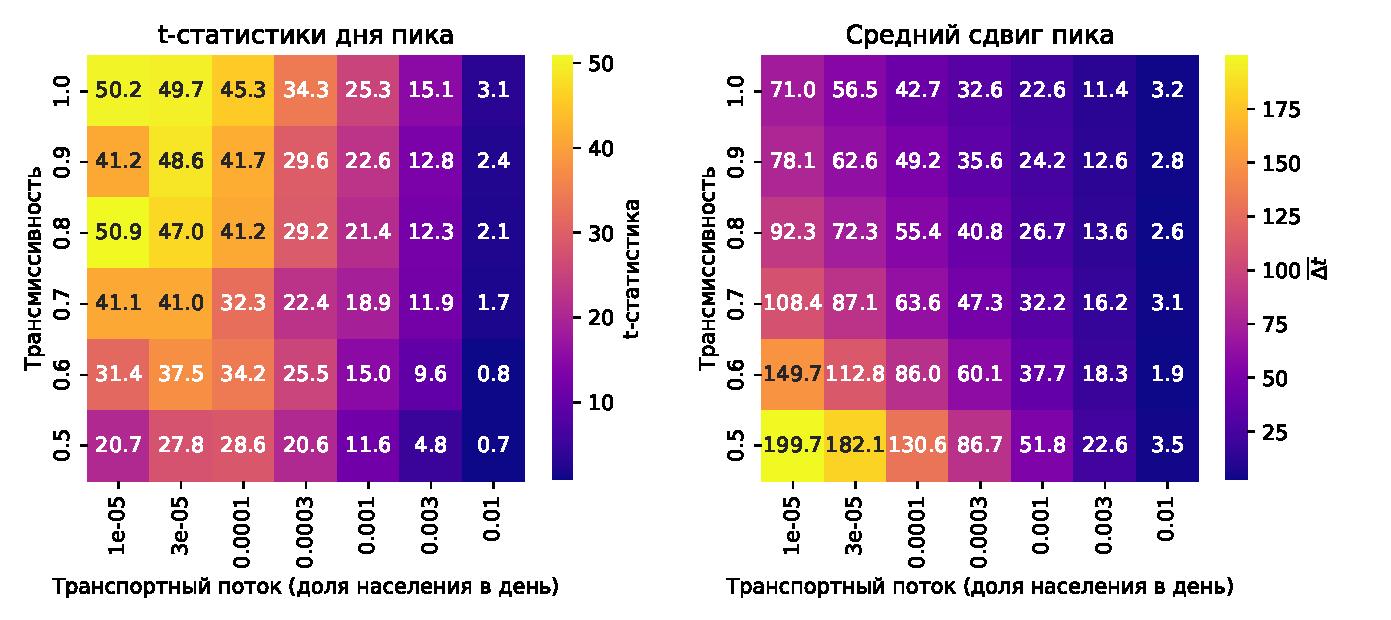
\includegraphics[width=0.95\linewidth]{images/flows_heatmap_conference.pdf}
    \caption{Тепловые карты среднего сдвига дня пика (слева) и t-статистики сдвига дня пика (справа).}
    \label{pic:flows_heatmap_conference}
\end{figure}

\begin{figure}[H]
    \centering
    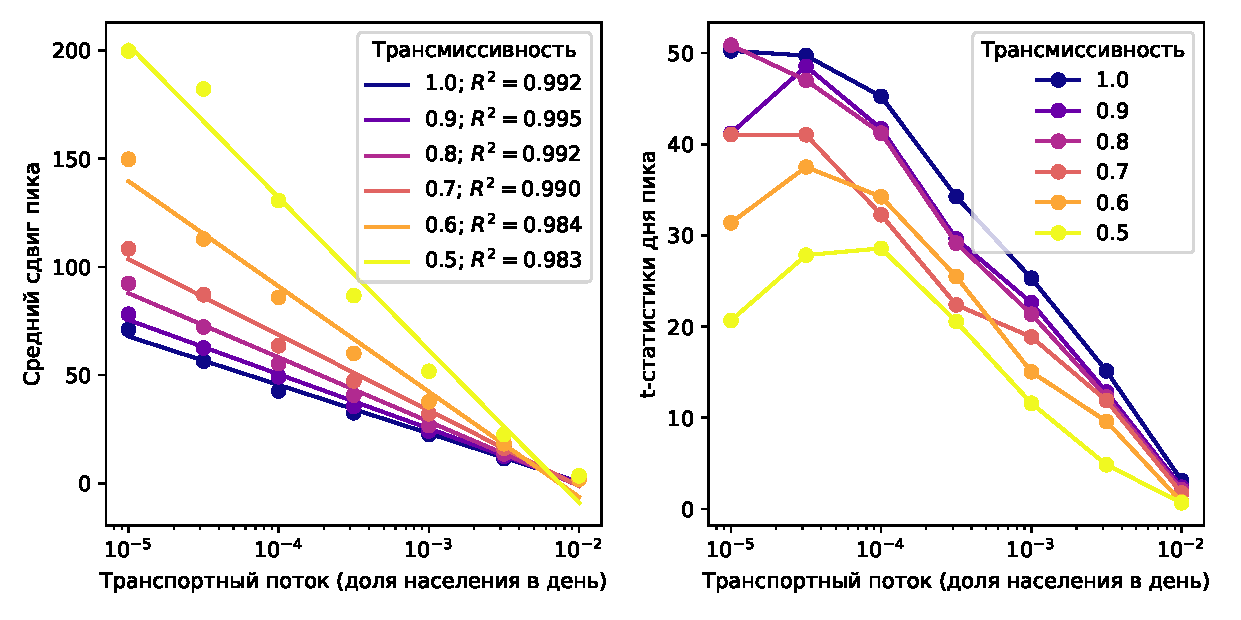
\includegraphics[width=0.95\linewidth]{images/flows_lines.pdf}
    \caption{Зависимости среднего сдвига дня пика (слева) и t-статистики сдвига дня пика (справа) от величины транспортного потока.}
    \label{pic:flows_lines}
\end{figure}


\newpage
\subsection{Индексы Соболя транспортных потоков модели двух городов}
Данный эксперимент ставился на модели двух городов с суммарным числом агентов 200 тысяч при различных размерах популяций. Проводилось вычисление индексов Соболя первого порядка потока из города начала и в город начала в отношении различных метрик эпидемии (кумулятивное число инфицирований, максимальное число инфицирований, день пика инфицирований) в исследуемых городах по 4096 точкам двумерной последовательности Соболя.

Минимальным исследуемым размером популяции города начала было 10 тысяч агентов. Схематичный вид модели транспортных потоков представлен на Рис. \ref{pic:bignsmall_small_start}. 

Наблюдается, что в такой системе исследуемые метрики практически не зависят от величины пассажиропотока из города начала ($S < 0.05$). При этом кумулятивное число инфицирований в городе начала возрастает с увеличением величины транспортного потока в него и индекс Соболя $S = 0.97\pm 0.08$. Максимальное же число инфицирований обладает таким же характером монотонности, а $S = 0.53\pm 0.08$. Эти зависимости представлены на Рис. \ref{pic:bignsmall_10000_0}. Помимо этого кумулятивное число инфицирований в соседнем городе убывает с увеличением потока из него ($S = 0.71\pm 0.07$), а день пика инфицирований в нем есть нелинейная убывающая функция потока из него ($S = 0.69\pm 0.08$). При этом метрики соседнего города также не зависят от потока из города начала ($S < 0.1$). Максимальное число инфицирований соседнего города не зависит ни от одного из рассматриваемых потоков ($S < 0.1$). Эти зависимости приведены на Рис. \ref{pic:bignsmall_10000_1}.

\begin{figure}[H]
    \centering
    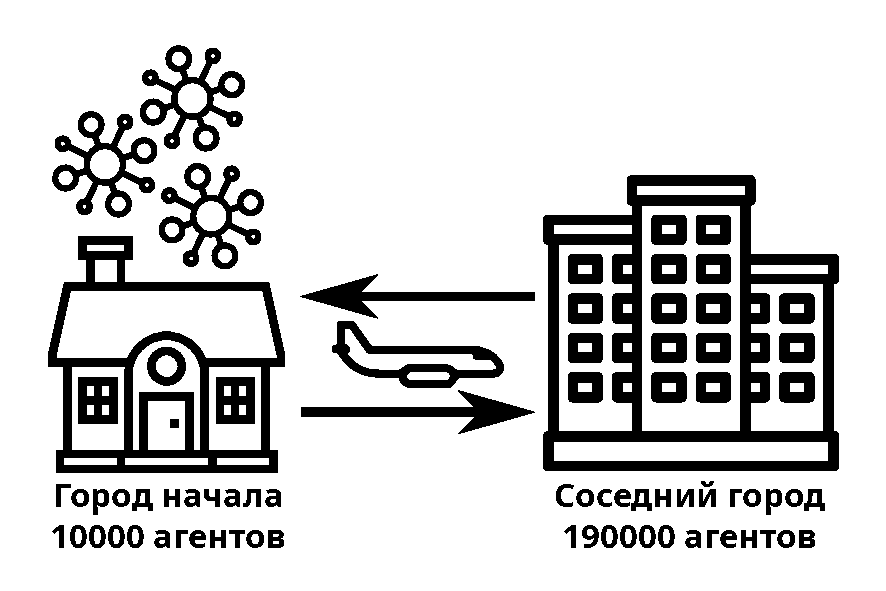
\includegraphics[width=0.5\linewidth]{images/bignsmall_small_start.pdf}
    \caption{Схематичное представление модели транспортных потоков при минимальном размере города начала в эксперименте по нахождению индексов Соболя транспортных потоков.}
    \label{pic:bignsmall_small_start}
\end{figure}




%\begin{table}[H]
%\begin{tabular}{|c|c|c|c|}
%\hline
                                                                                                    %& \begin{tabular}[c]{@{}c@{}}Кумулятивные \\ инфицирования\end{tabular} & \begin{tabular}[c]{@{}c@{}}Максимальное\\ число инфицирований\end{tabular} & День пика      \\ \hline
%\begin{tabular}[c]{@{}c@{}}Индекс Соболя первого порядка \\ потока из города начала\end{tabular}    & $0.011\pm 0.016$                                                      & $0.03\pm 0.06$                                                             & $0.00\pm 0.08$ \\ \hline
%\begin{tabular}[c]{@{}c@{}}Индекс Соболя первого порядка \\ потока из соседнего города\end{tabular} & $0.97\pm 0.08$                                                        & $0.53\pm 0.08$                                                             & $0.13\pm 0.08$ \\ \hline
%\end{tabular}
%\caption{Индексы Соболя транспортных потоков при вычислении различных метрик эпидемии в городе начала при его минимальном размере.}
%\label{tab:bignsmall_10000_0}
%\end{table}

\begin{figure}[H]
    \centering
    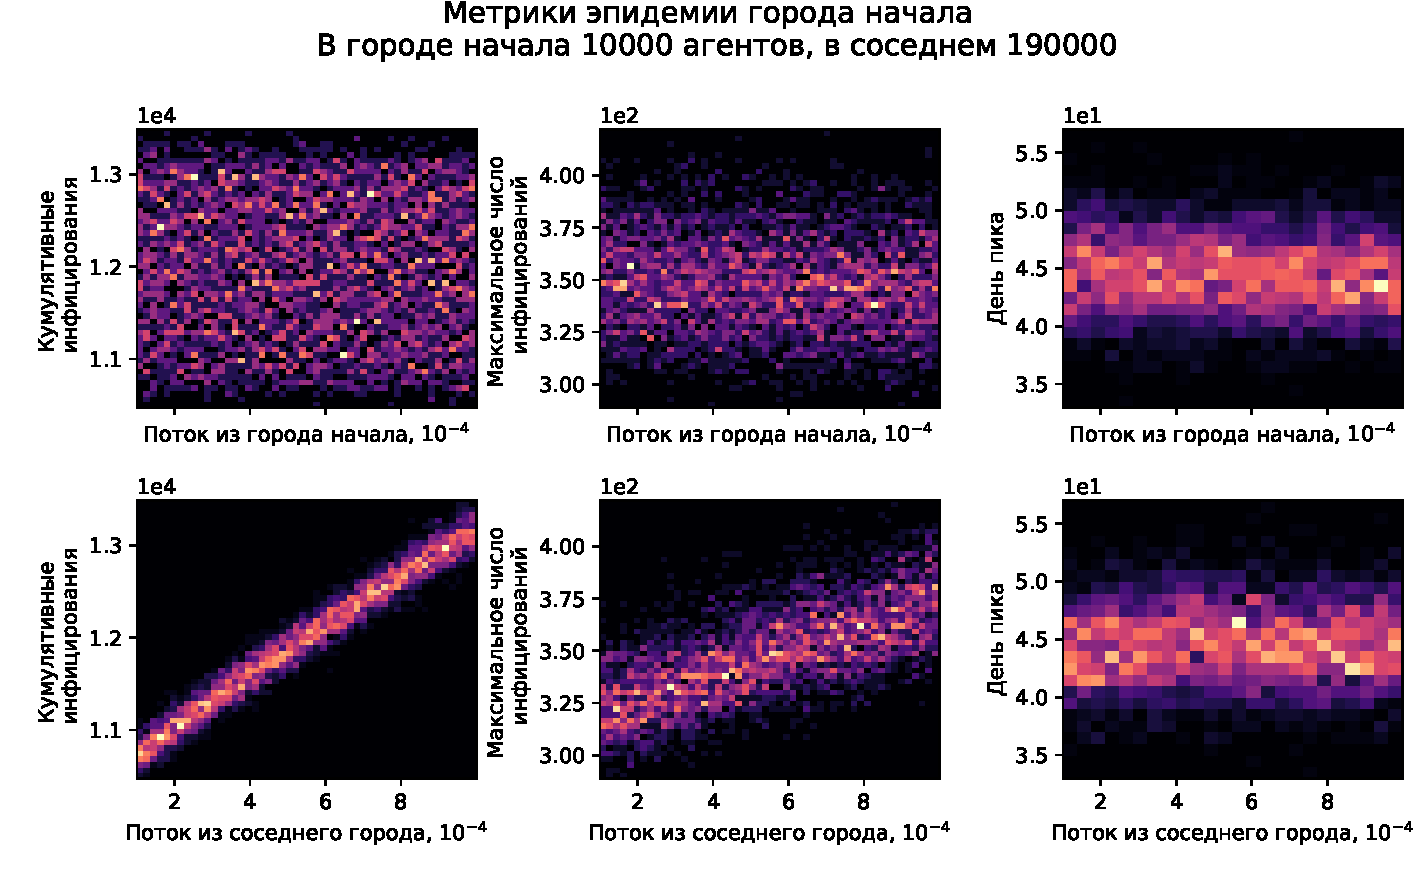
\includegraphics[width=0.9\linewidth]{images/bignsmall_10000_0.pdf}
    \caption{Тепловые карты зависимости различных метрик эпидемии города начала от транспортных потоков модели при минимальном рассматриваемом размере города начала.}
    \label{pic:bignsmall_10000_0}
\end{figure}








%\begin{table}[H]
%\begin{tabular}{|c|c|c|c|}
%\hline
                                                                                                    %& \begin{tabular}[c]{@{}c@{}}Кумулятивные \\ инфицирования\end{tabular} & \begin{tabular}[c]{@{}c@{}}Максимальное\\ число инфицирований\end{tabular} & День пика      \\ \hline
%\begin{tabular}[c]{@{}c@{}}Индекс Соболя первого порядка \\ потока из города начала\end{tabular}    & $0.00\pm 0.04$                                                        & $-0.09\pm 0.08$                                                            & $0.01\pm 0.04$ \\ \hline
%\begin{tabular}[c]{@{}c@{}}Индекс Соболя первого порядка \\ потока из соседнего города\end{tabular} & $0.71\pm 0.07$                                                        & $0.02\pm 0.08$                                                             & $0.69\pm 0.08$ \\ \hline
%\end{tabular}
%\caption{Индексы Соболя транспортных потоков при вычислении различных метрик эпидемии в соседнем городе при минимальном размере города начала.}
%\label{tab:bignsmall_10000_1}
%\end{table}



\begin{figure}[H]
    \centering
    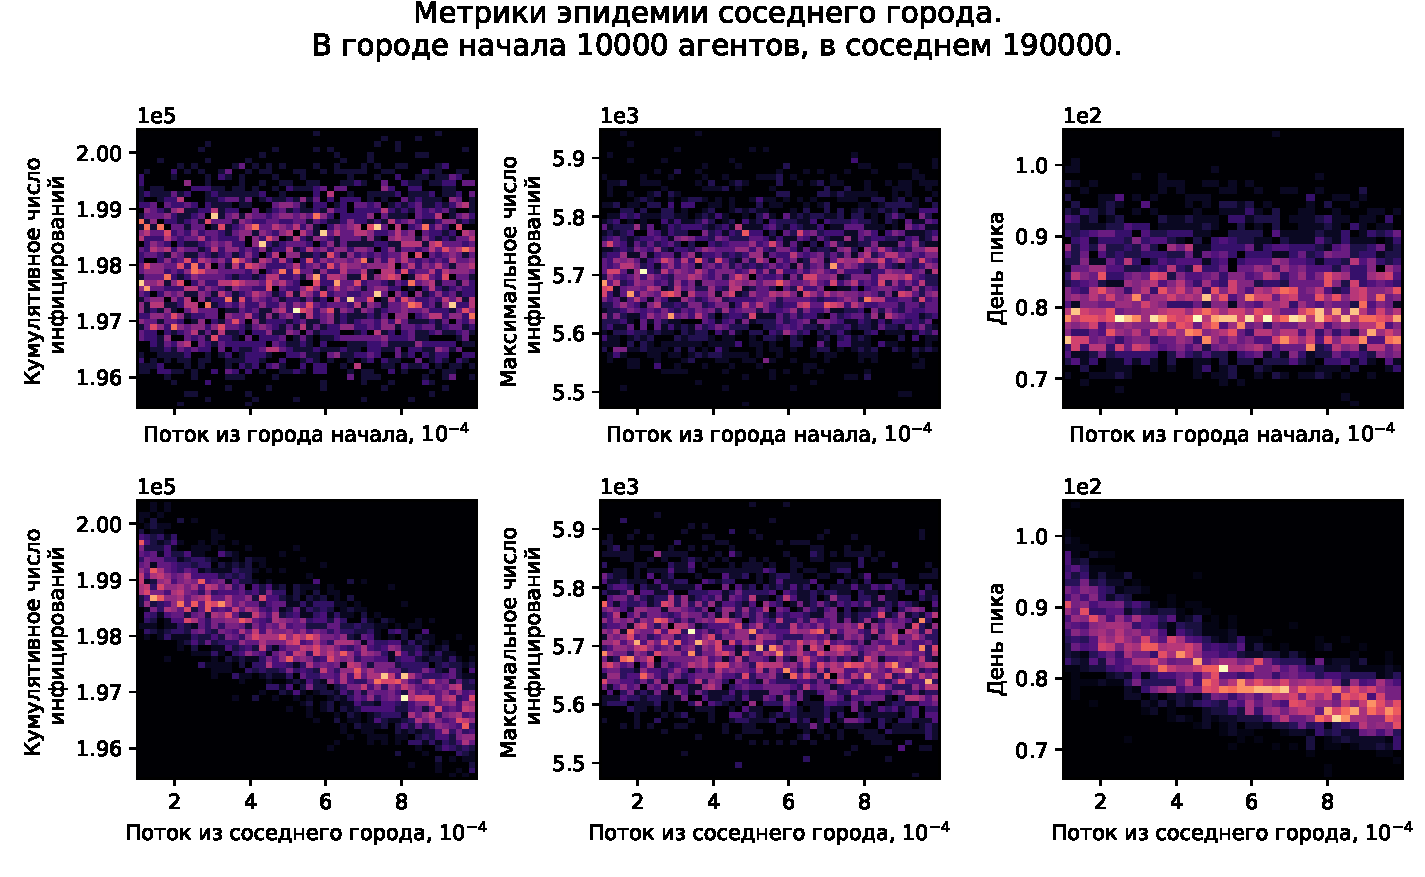
\includegraphics[width=0.9\linewidth]{images/bignsmall_10000_1.pdf}
    \caption{Тепловые карты зависимости различных метрик эпидемии соседнего города от транспортных потоков модели при минимальном рассматриваемом размере города начала.}
    \label{pic:bignsmall_10000_1}
\end{figure}

Максимальный исследуемый размер популяции города начала --- 190 тысяч агентов, при этом в соседнем городе --- 10 тысяч. Модель транспортных потоков в данном случае приведена на Рис. \ref{pic:bignsmall_big_start}. 

В отличие от предыдущей модели в данном случае метрики практически не зависят от потоков из соседнего города ($S < 0.05$). Теперь кумулятивное число инфицирований и максимальное число инфицирований города начала убывают с ростом потока из него ($S$ соответственно $0.45\pm 0.09$, $0.14\pm 0.10$). Кумулятивное и максимальное число инфицирований соседнего города возрастает с увеличением потока из города начала, а день наступления пика убывает ($S$ соответственно $0.88\pm 0.08$, $0.66\pm 0.07$, $0.58\pm 0.08$). Эти результаты приведены на Рис. \ref{pic:bignsmall_190000_0}, \ref{pic:bignsmall_190000_1}.

\begin{figure}[H]
    \centering
    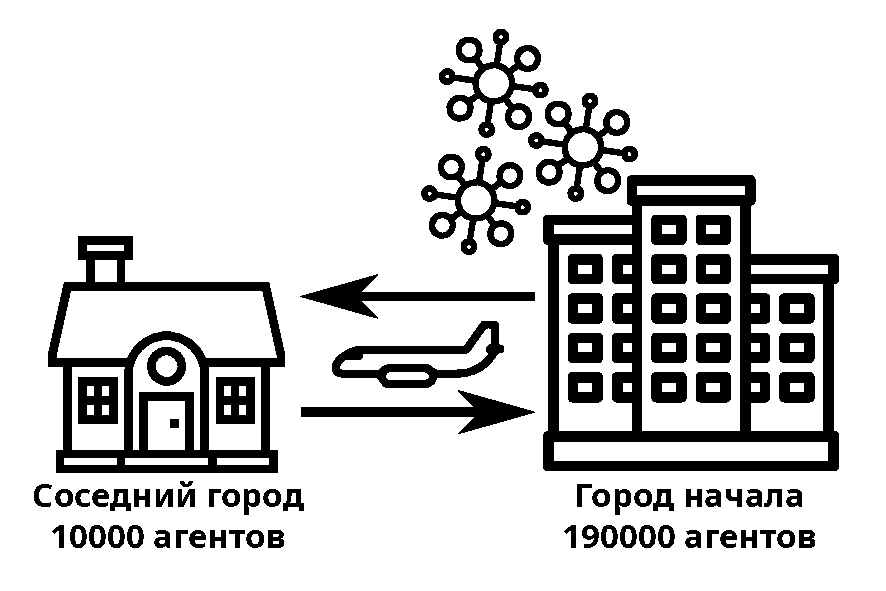
\includegraphics[width=0.5\linewidth]{images/bignsmall_big_start.pdf}
    \caption{Схематичное представление модели транспортных потоков при максимальном размере города начала в эксперименте по нахождению индексов Соболя транспортных потоков.}
    \label{pic:bignsmall_big_start}
\end{figure}


%\begin{table}[H]
%\begin{tabular}{|c|c|c|c|}
%\hline
                                                                                                    %& \begin{tabular}[c]{@{}c@{}}Кумулятивные \\ инфицирования\end{tabular} & \begin{tabular}[c]{@{}c@{}}Максимальное\\ число инфицирований\end{tabular} & День пика       \\ \hline
%\begin{tabular}[c]{@{}c@{}}Индекс Соболя первого порядка \\ потока из города начала\end{tabular}    & $0.45\pm 0.09$                                                        & $0.14\pm 0.10$                                                             & $0.50\pm 0.08$  \\ \hline
%\begin{tabular}[c]{@{}c@{}}Индекс Соболя первого порядка \\ потока из соседнего города\end{tabular} & $-0.01\pm 0.07$                                                       & $-0.04\pm 0.08$                                                            & $-0.01\pm 0.06$ \\ \hline
%\end{tabular}
%\caption{Индексы Соболя транспортных потоков при вычислении различных метрик эпидемии в городе начала при его максимальном размере.}
%\label{tab:bignsmall_190000_0}
%\end{table}

\begin{figure}[H]
    \centering
    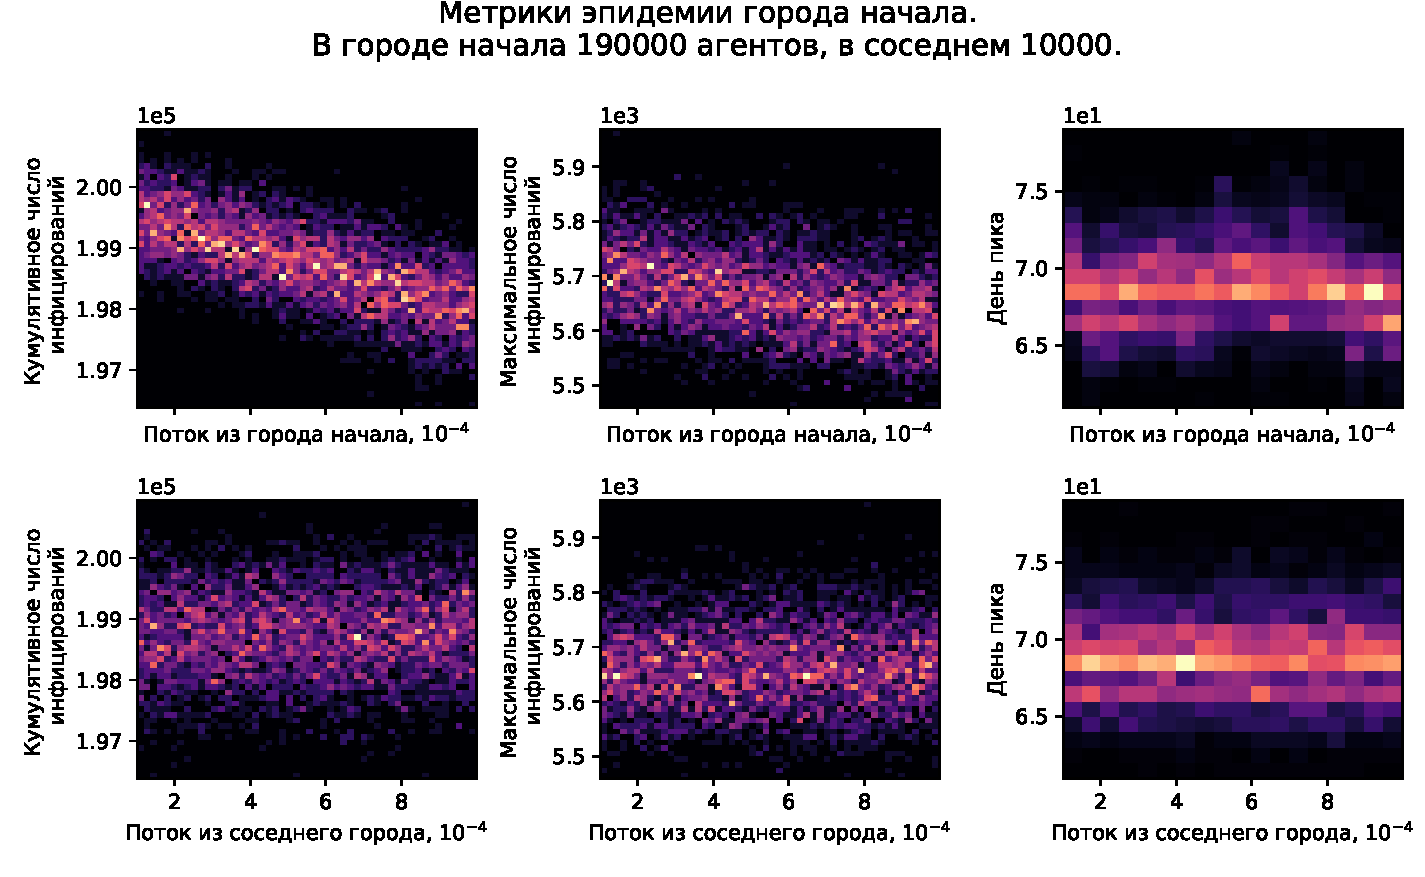
\includegraphics[width=0.9\linewidth]{images/bignsmall_190000_0.pdf}
    \caption{Тепловые карты зависимости различных метрик эпидемии города начала от транспортных потоков модели при максимальном рассматриваемом размере города начала.}
    \label{pic:bignsmall_190000_0}
\end{figure}


%\begin{table}[H]
%\begin{tabular}{|c|c|c|c|}
%\hline
                                                                                                    %& \begin{tabular}[c]{@{}c@{}}Кумулятивные \\ инфицирования\end{tabular} & \begin{tabular}[c]{@{}c@{}}Максимальное\\ число инфицирований\end{tabular} & День пика      \\ \hline
%\begin{tabular}[c]{@{}c@{}}Индекс Соболя первого порядка \\ потока из города начала\end{tabular}    & $0.88\pm 0.08$                                                        & $0.66\pm 0.07$                                                             & $0.58\pm 0.08$ \\ \hline
%\begin{tabular}[c]{@{}c@{}}Индекс Соболя первого порядка \\ потока из соседнего города\end{tabular} & $0.00\pm 0.02$                                                        & $0.00\pm 0.05$                                                             & $0.00\pm 0.05$ \\ \hline
%\end{tabular}
%\caption{Индексы Соболя транспортных потоков при вычислении различных метрик эпидемии в соседнем городе при максимальном размере города начала.}
%\label{tab:bignsmall_190000_1}
%\end{table}

\begin{figure}[H]
    \centering
    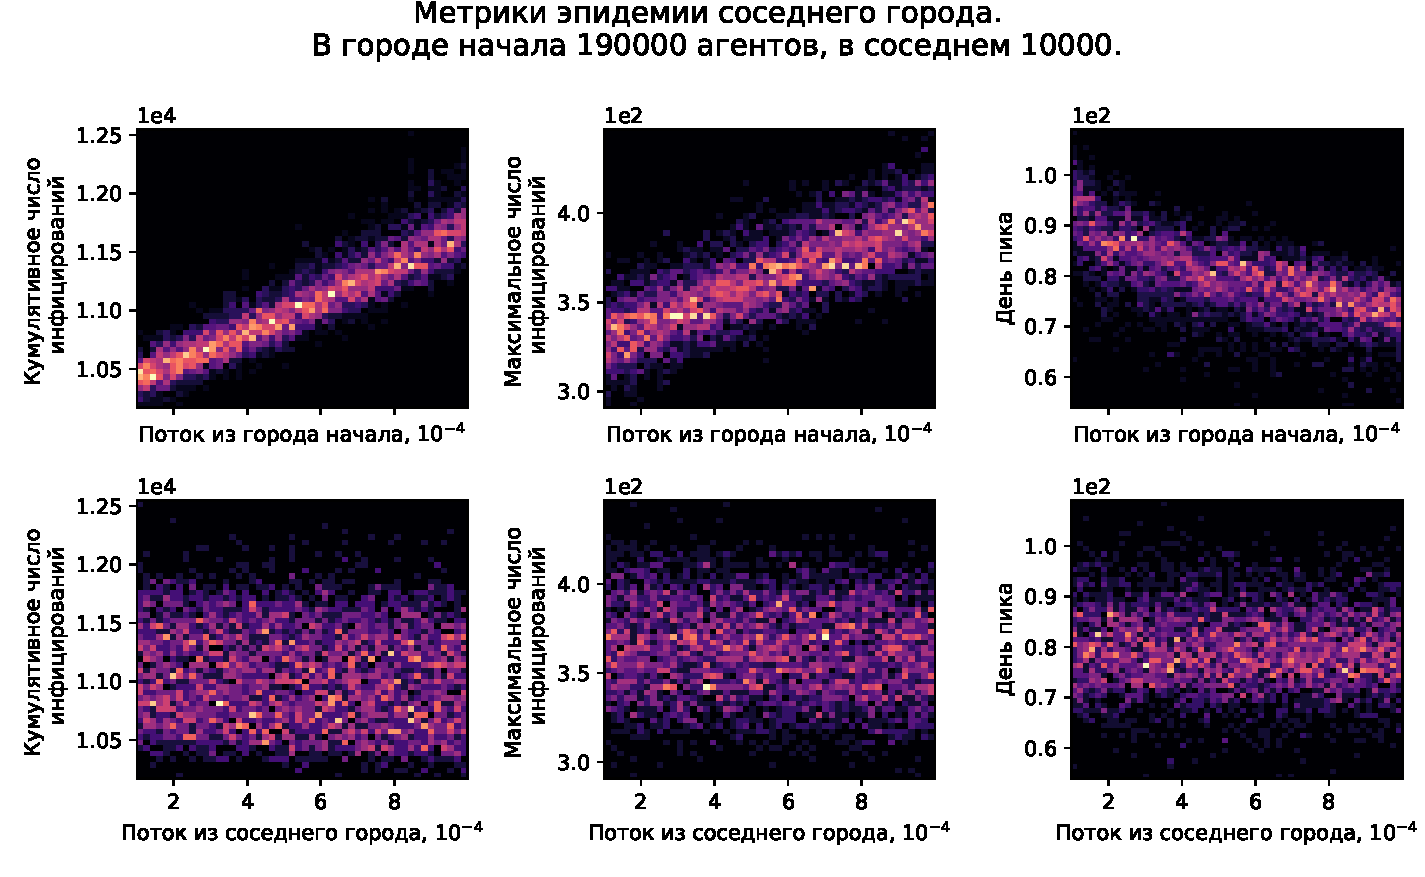
\includegraphics[width=0.9\linewidth]{images/bignsmall_190000_1.pdf}
    \caption{Тепловые карты зависимости различных метрик эпидемии соседнего города от транспортных потоков модели при максимальном рассматриваемом размере города начала.}
    \label{pic:bignsmall_190000_1}
\end{figure}

Индексы Соболя исследуемых метрик при промежуточных соотношениях размеров популяций городов приведены на Рис. \ref{pic:bignsmall_bars}. Наблюдается, что с увеличением размера популяции города начала чувствительность кумулятивного числа инфицирований для обеих городов к потоку из города начала растет, а в город начала --- убывает. 

При этом максимальное число инфицирований практически не зависит от потока из соответствующего города ($S < 0.25$). Также для соседнего города чувствительность максимального числа инфицирований от потока из города начала монотонно возрастает с увеличением размера города начала, а чувствительность для города начала к потоку в него резко убывает так, что при размере популяции города начала большей 50 тысяч агентов практически нулевая ($S < 0.2$). 

Чувствительность дня пика инфицирований в соседнем городе к потоку из города начала убывает, а из соседнего города возрастает с увеличением размера города начала. День пика в городе начала практически не зависит от потока в него ($S < 0.2$).

\begin{figure}[H]
    \centering
    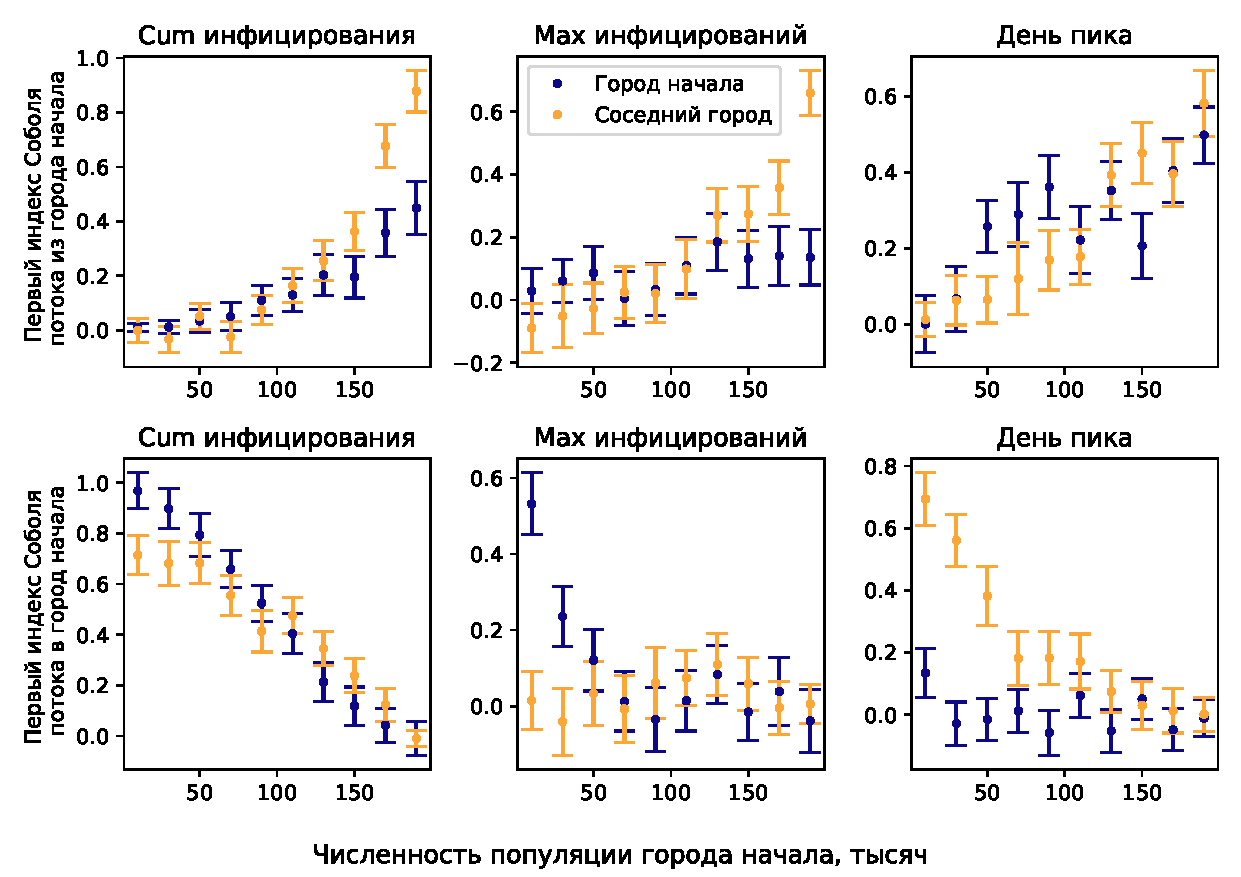
\includegraphics[width=\linewidth]{images/bignsmall_bars.pdf}
    \caption{Индексы Соболя транспортных потоков по отношению к различным метрикам эпидемии в городе начала и соседнем городе.}
    \label{pic:bignsmall_bars}
\end{figure}


\subsection{Модель трудовой миграции в системе пяти городов (<<Хаб и сателлиты>>)}
В данном эксперименте была построена модель пассажиропотоков хаб-сателлиты. Хаб --- большой центральный город, вокруг которого сформированы более мелкие города-сателлиты. Отношение количеств агентов в хабе и сателлитах соответствует отношению численностей населения Москвы и Московской области, суммарное число агентов в 20 раз меньше суммарного числа людей для сокращения длительности расчетов. Область разделена на 4 города. Транспортный поток из хаба в сателлиты и из сателлитов в хаб соответствует данным операторов сотовой связи, взятым из \cite{makhrova2017work}. Остальные потоки оценены из гравитационной модели, предполагающей пропорциональность потоков численностям популяций и обратную их пропорциональность квадрату расстояния между городами (частный случай модели, рассмотренной в разделе <<Обзор литературы>>). Для простоты хаб предполагался располагающимся в центре квадрата с вершинами в сателлитах (то есть расстояние между соседними сателлитами в $\sqrt{2}$ раз больше расстояния хаб-сателлиты, а между противоположными --- в 2 раза). Время нахождения агента в городе назначения было равно 1 дню, число контактов --- 40, множитель трансмиссивности слоя туристов --- 0.6, что соответствует взаимодействиям людей при перемещениях в соседние города на свои рабочие места. Модель транспортных потоков в данной системе приведена на Рис. \ref{pic:graph1}. 


\begin{figure}[H]
    \centering
    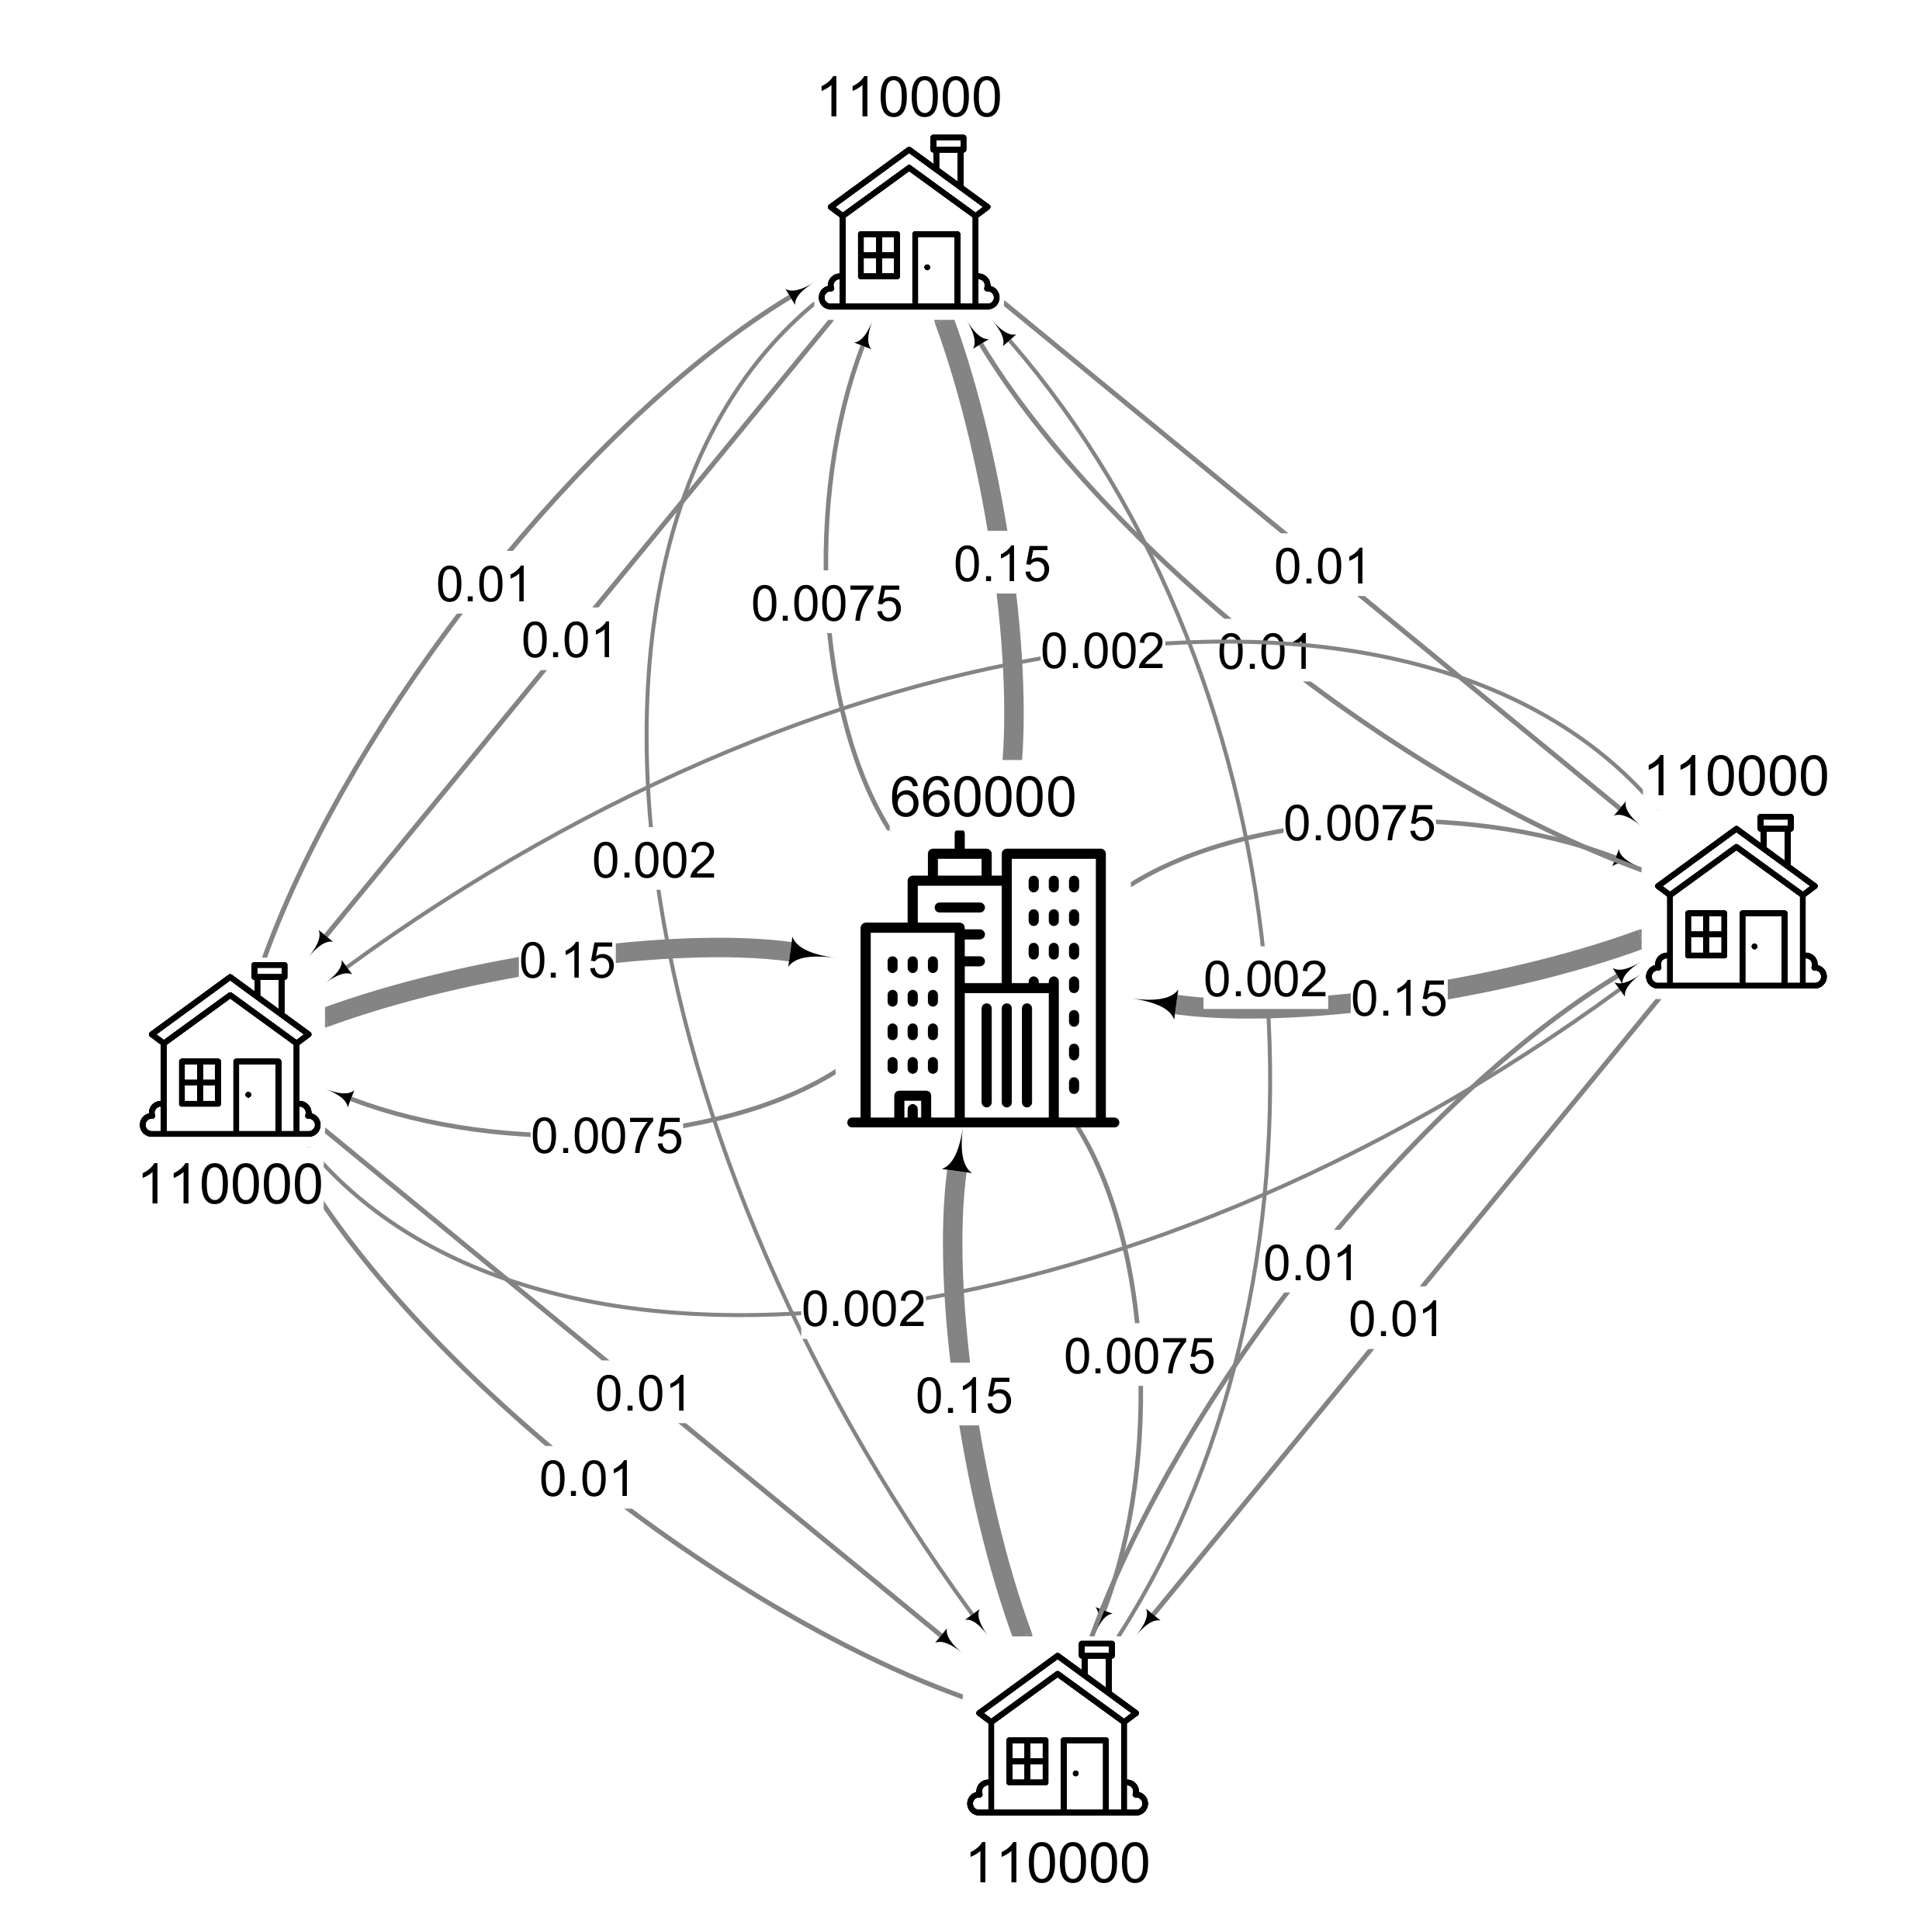
\includegraphics[width=0.6\linewidth]{images/graph1.png}
    \caption{Представление рассматриваемой модели транспортных потоков в системе хаб-сателлиты в виде графа (подписи у вершин --- количество агентов в популяции населенного пункта, у ребер --- доля населения города, ежедневно отправляющаяся в однодневную поездку в соответствии с положением ребра).}
    \label{pic:graph1}
\end{figure}

Запускались по 30 симуляций при начале эпидемии в сателлите и в хабе, после чего на различных шагах симуляции вводились ограничения: уменьшение в 10 или в 100 раз всех транспортных потоков системы или уменьшение в 10 или 100 раз потоков на дорогах, непосредственно связанных с городом начала. Также для сравнения были запущены по 30 симуляций в отсутствие ограничений. По результатам вычислений определялись исследуемые метрики: максимальное число ежедневных инфицирований, критических случаев, смертей, а также день пика инфицирований.

На Рис. \ref{pic:satellites_hists0} приведены зависимости исследуемых метрик системы от дня введения эпидемиологических мер и их вида при начале эпидемии в хабе. Серой полосой отмечены метрики и их среднеквадратичные отклонения по 30 симуляциям без введения ограничений. Доверительный интервал отмечен звездой, если разница наблюдаемой метрики в присутствие ограничений и в отсутствие является статистически значимой при тесте Стьюдента при пороговом уровне значимости 0.05 (с поправкой на множественные сравнения). Для иллюстрации положения дня введения мер на Рис. \ref{pic:satellites_epid0} приведены эпидемиологические кривые системы при начале эпидемии в хабе (слева) и сателлите (справа).

Эксперименты показали, что при начале эпидемии в хабе введение ограничений вплоть до дня пика эпидемии позволяет достигнуть статистически значимого снижения пиковых чисел инфицированных, критических случаев, смертей. При введении ограничений с 40 по 70 день (в конце экспоненциальной фазы) эпидемии разница между уменьшением потоков в 10 и 100 раз между всеми городами или только между хабом и сателлитами незначительна, также эффект от введения этих мер практически не меняется в конце экспоненциальной фазы, это проиллюстрировано на Рис. \ref{pic:satellites_hists0}. Даже при введении мер в это время удается достичь снижения пиковых чисел зараженных на $10\%$ ($p = 10^{-49}$), критических случаев на $20\%$ ($p = 10^{-36}$), смертей на $20\%$ ($p = 10^{-25}$). Разница между ограничением потоков в 10 и 100 раз наблюдается на ранних этапах эпидемии --- там ограничения пассажиропотоков в 100 раз позволяют уменьшить пиковые значения еще практически в два раза в сравнении с введением в конце экспоненциальной фазы.

На Рис. \ref{pic:satellites_hists1} приведены аналогичные зависимости при начале эпидемии в сателлите. Ключевой разницей является тот факт, что ограничения только на потоки, связанные с этим сателлитом, намного менее эффективны, чем ограничения на все потоки, хотя снижение целевых метрик и является статистически значимым.

\begin{figure}[H]
    \centering
    \begin{subfigure}{0.45\linewidth}
        \centering
        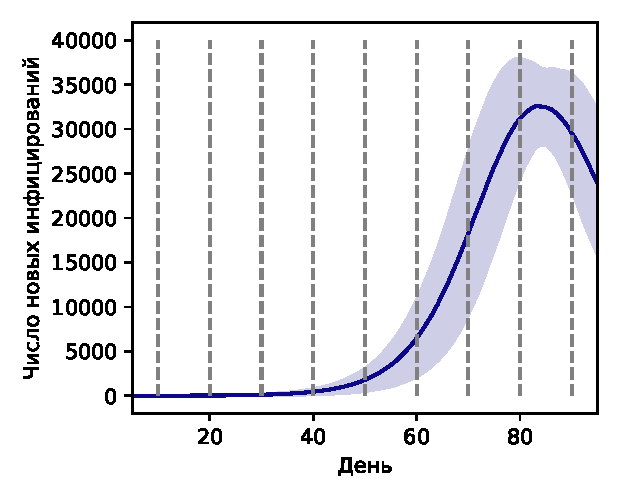
\includegraphics[width=\linewidth]{images/satellites_epid0.pdf}
    \end{subfigure}
    \hfill
    \begin{subfigure}{0.45\linewidth}
        \centering
        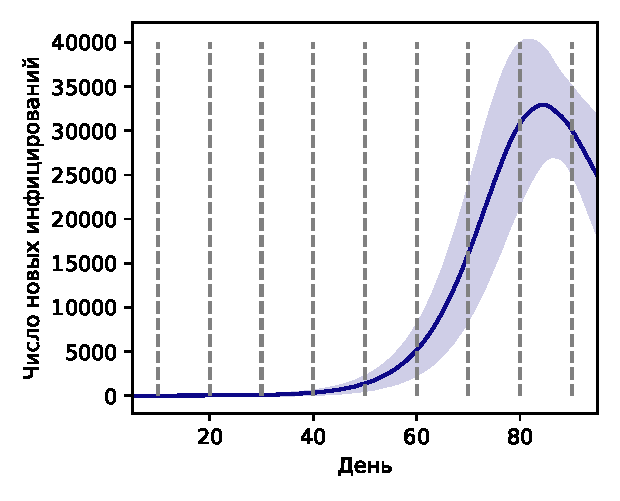
\includegraphics[width=\linewidth]{images/satellites_epid1.pdf}
    \end{subfigure}
    \caption{Суммарное число новых ежедневных инфицирований в системе при моделировании в отсутствие ограничительных мер при начале эпидемии в хабе (слева) и сателлите (справа) (заполнение цветом соответствует среднеквадратичному отклонению по результатам 30 запусков симуляции).}
    \label{pic:satellites_epid0}
\end{figure}

\begin{figure}[H]
    \centering
    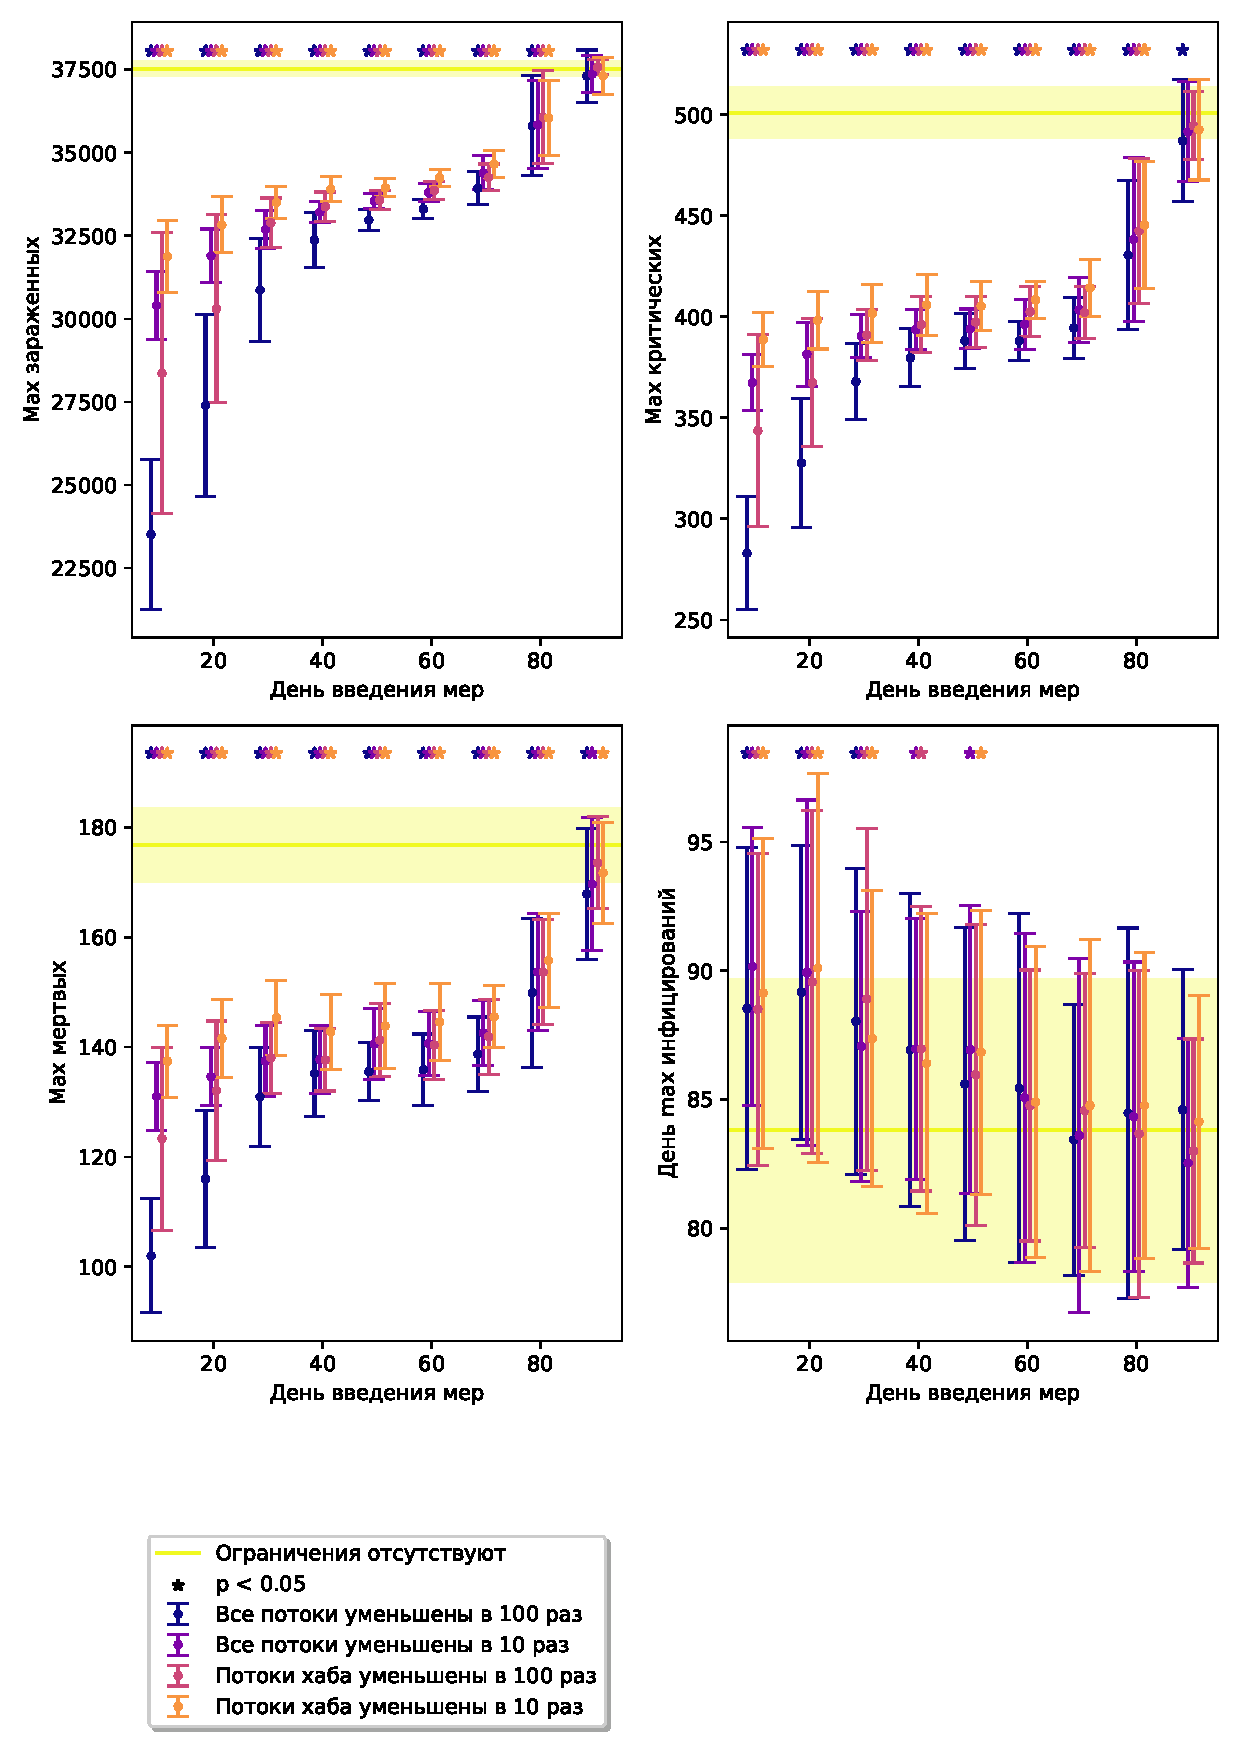
\includegraphics[width=\linewidth]{images/satellites_hists0.pdf}
    \caption{Зависимости исследуемых метрик системы от дня введения ограничений на транспортные потоки и величины этих ограничений при начале эпидемии в хабе.}
    \label{pic:satellites_hists0}
\end{figure}

\begin{figure}[H]
    \centering
    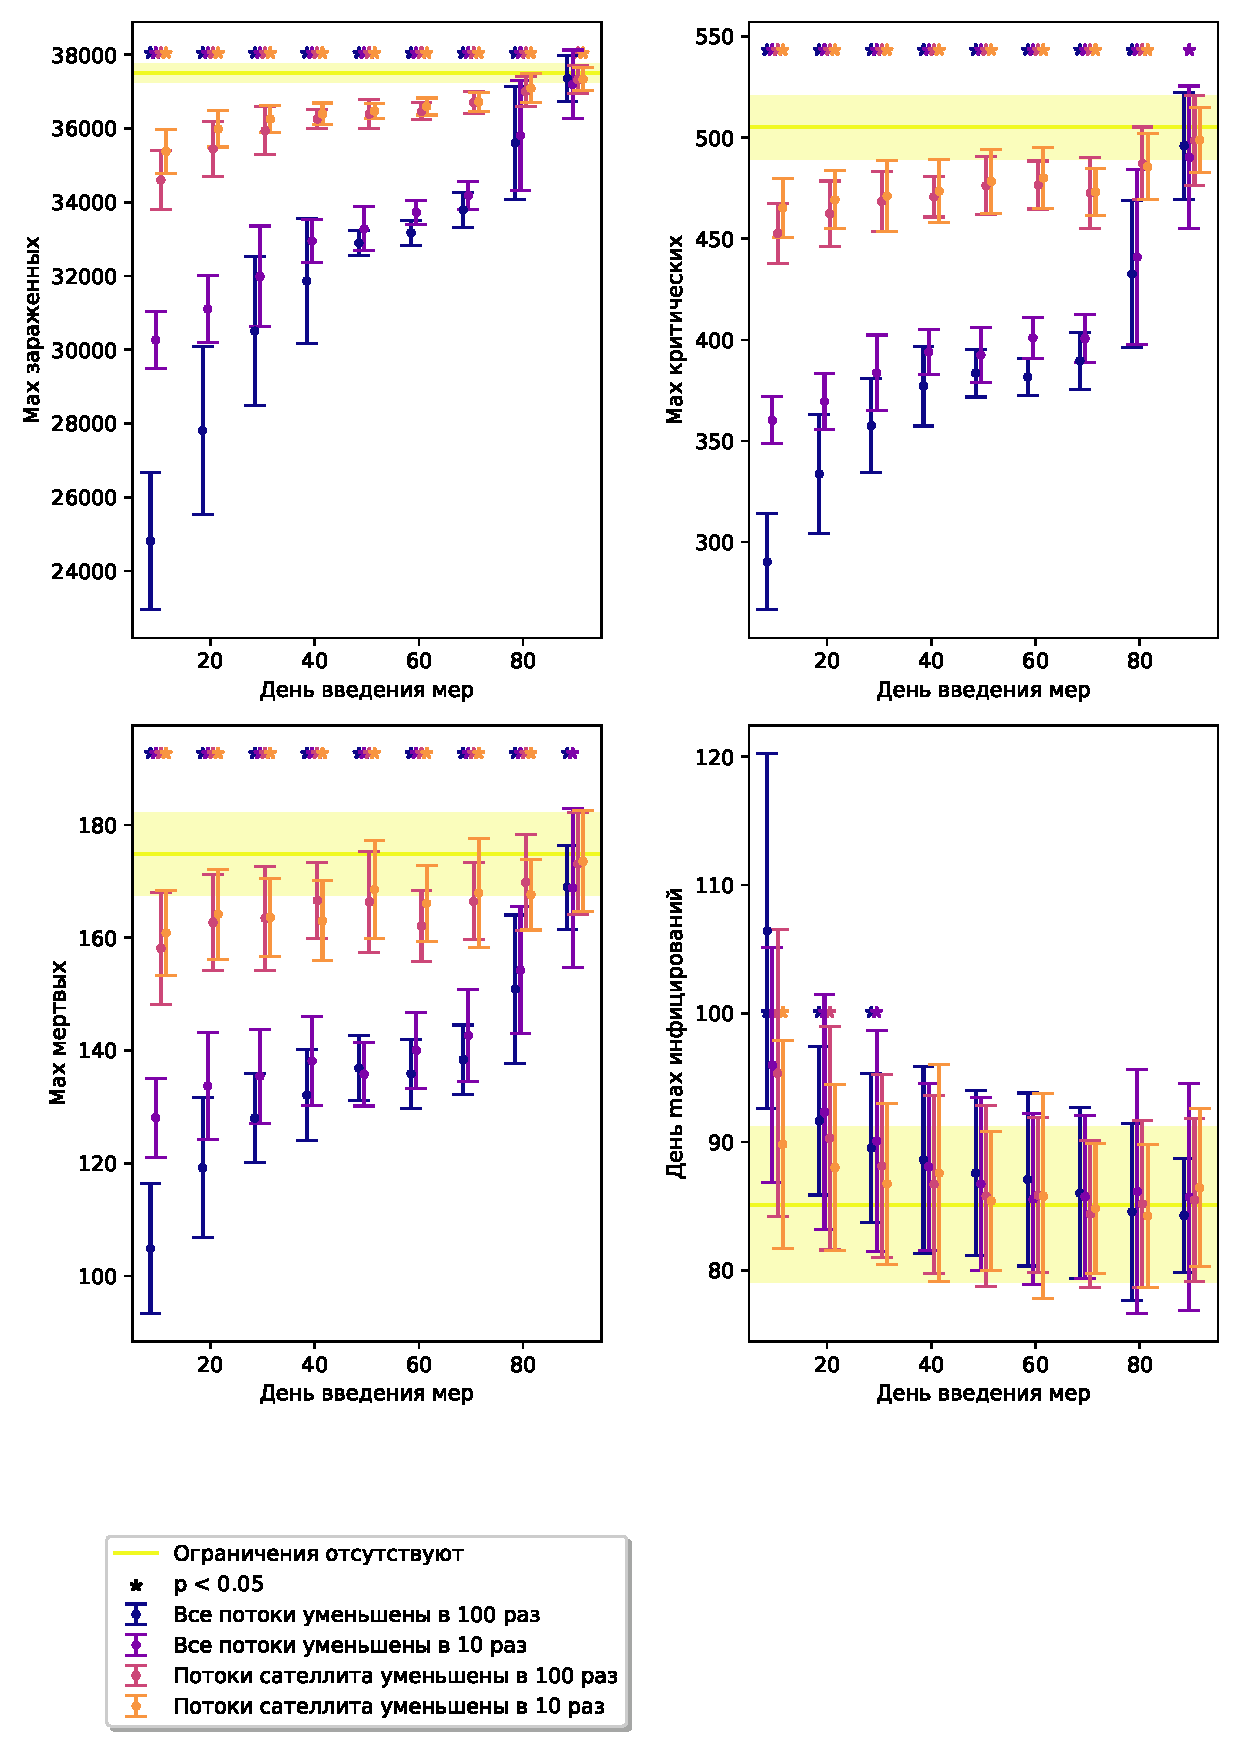
\includegraphics[width=\linewidth]{images/satellites_hists1.pdf}
    \caption{Зависимости исследуемых метрик системы от дня введения ограничений на транспортные потоки и величины этих ограничений при начале эпидемии в сателлите.}
    \label{pic:satellites_hists1}
\end{figure}

На Рис. \ref{pic:satellites_boxs} изображены те же метрики, но для отдельных городов при начале эпидемии в сателлите и в хабе в отсутствие ограничений. Звездой отмечена статистически значимая разница метрик города при начале в хабе и в сателлите. Оказалось, что в подобной системе детектировать место начала эпидемии по рассматриваемым метрикам не представляется возможным. Это также иллюстрирует Рис. \ref{pic:satellites_epids0}.

\begin{figure}[H]
    \centering
    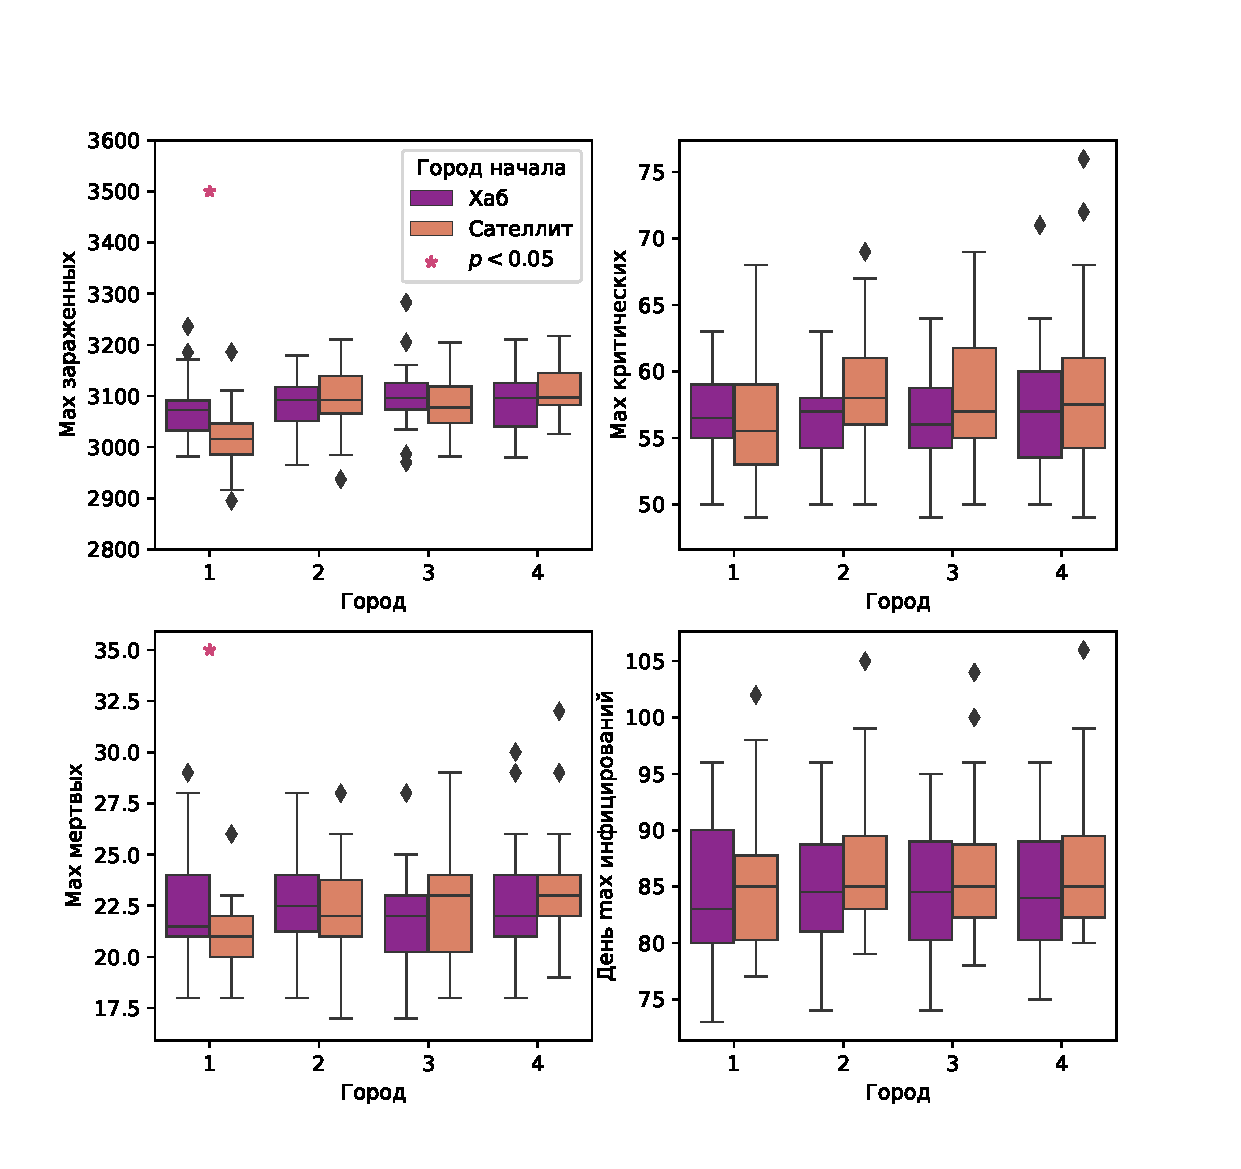
\includegraphics[width=\linewidth]{images/satellites_boxs.pdf}
    \caption{Исследуемые метрики в различных сателлитах в зависимости от места начала эпидемии (ограничительные меры отсутствуют).}
    \label{pic:satellites_boxs}
\end{figure}

\begin{figure}[H]
    \centering
    \begin{subfigure}{0.45\linewidth}
        \centering
        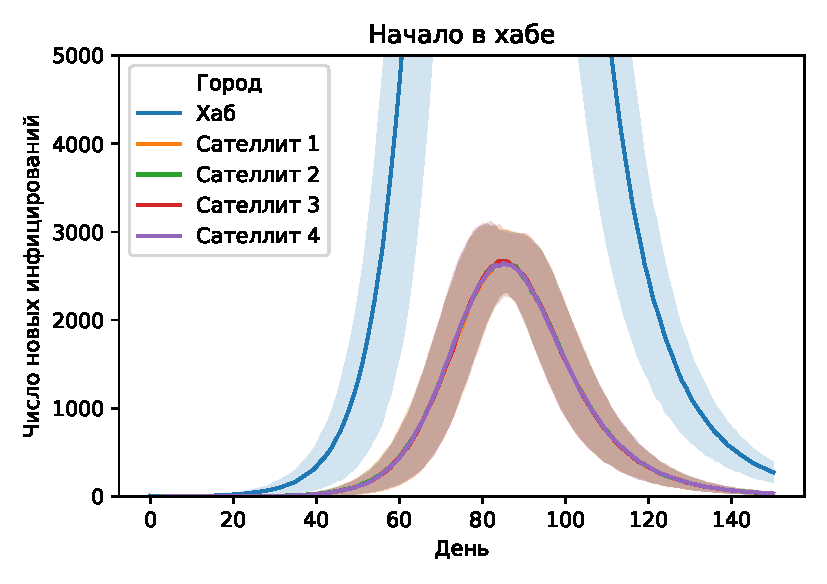
\includegraphics[width=\linewidth]{images/satellites_epids0.pdf}
    \end{subfigure}
    \hfill
    \begin{subfigure}{0.45\linewidth}
        \centering
        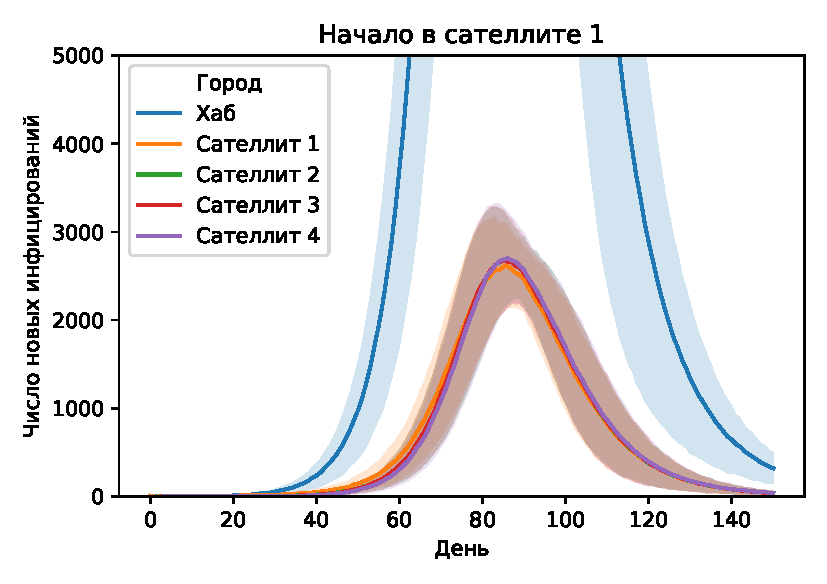
\includegraphics[width=\linewidth]{images/satellites_epids1.pdf}
    \end{subfigure}
    \caption{Суммарное число новых ежедневных инфицирований в отдельных городах в системе хаб-сателлиты при моделировании в отсутствие ограничительных мер при начале эпидемии в хабе (слева) и в сателлите (справа).}
    \label{pic:satellites_epids0}
\end{figure}



\subsection{Детекция города начада эпидемии в модели <<хаб-сателлиты>>}

Эксперименты проводились над моделью транспортных потоков хаб-сателлиты, описанной выше, при различных значениях трансмиссивности инфекции и множителя на все величины транспортных потоков. Эпидемиологические кривые для различных сателлитов усреднялись, после чего вычислялось среднее абсолютное отклонение (MAE) этих кривых от средней, нормированное на максимум кривой. Распределение сравниваемых метрик проверялось на нормальность тестом Шапиро-Уилка. В связи с несоответствием распределения метрики нормальному для сравнения результатов симуляции при начале эпидемии в хабе и в сателлите проводился тест Манна-Уитни.

Оказалось, что при начале в хабе, вне зависимости от скорости распространения инфекции в системе, эпидемиологические кривые сателлитов являются более синхронными при всех рассматриваемых множителях транспортных потоков. Это продемонстрировано на Рис. \ref{pic:diffsatellites_demos}.

На Рис. \ref{pic:diffsatellites_heatmaps} приведены тепловые карты средней разницы нормированных значений MAE эпидемиологических кривых при симулировании начала эпидемии в сателлите и в хабе (слева) и p-значение при сравнении их распределений тестом Манна-Уитни (справа). Среднее значение --- монотонно убывающая функция множителя транспортного потока, p-значение --- немонотонная функция с максимумом вблизи множителя $3\cdot 10^{-2}$, что может быть связано с увеличением разброса результатов в этой области, являющимся проявлением дискретности модели на малых величинах транспортных потоков. 

При пороговом уровне значимости $p<0.05$ оказывается, что при трансмиссивности инфекции, соответствующей уханьскому варианту \gls{sars}, случаи начала эпидемии в хабе и сателлите удается уверенно различить, то есть предложенная нами в этом эксперименте метрика является более чувствительной для нашей задачи, чем стандартные, рассматриваемые в предыдущем эксперименте. Также при любых других рассматриваемых трансмиссивностях при множителе транспортного потока меньше единицы детекция города начала оказывается возможной. Эти результаты приведены на Рис. \ref{pic:diffsatellites_heatmaps}.
 

 
 \begin{figure}[H]
    \centering
    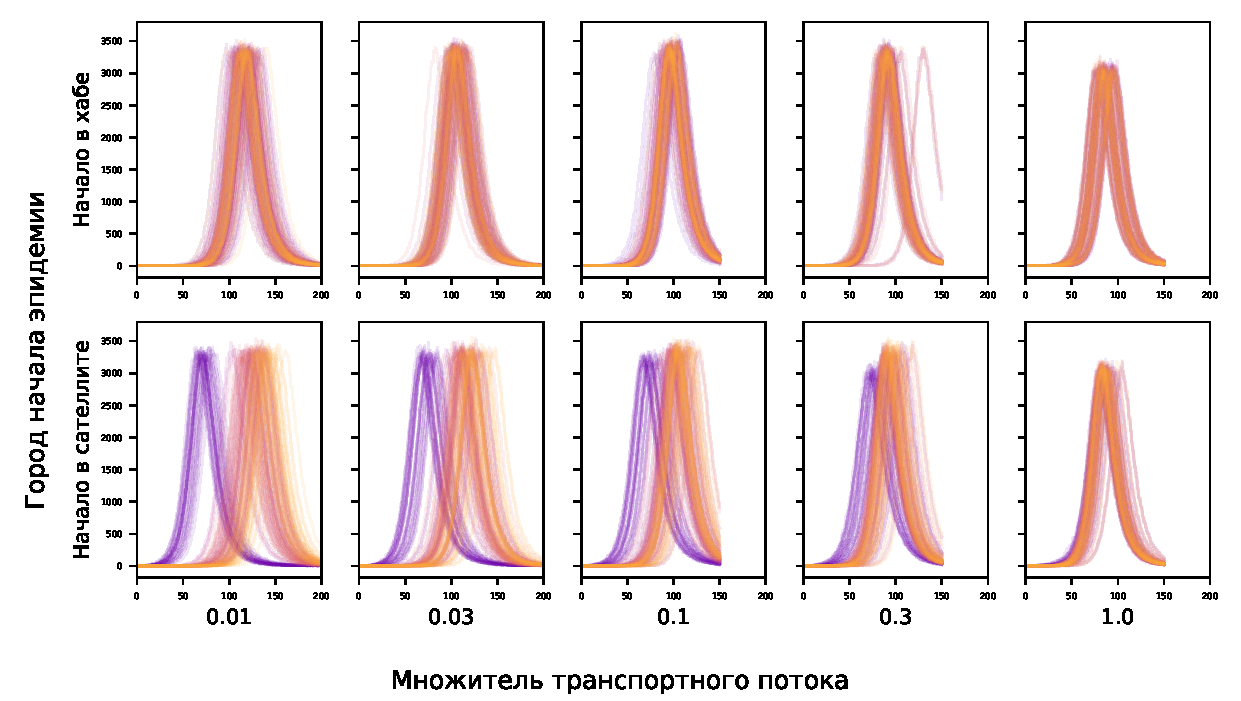
\includegraphics[width=\linewidth]{images/diffsatellites_demos.pdf}
    \caption{Эпидемиологические кривые различных сателлитов системы хаб-сателлиты при различных величинах множителя транспортного потока при начале эпидемии в хабе (сверху) и в сателлите 1 (снизу).}
    \label{pic:diffsatellites_demos}
\end{figure}

\begin{figure}[H]
    \centering
    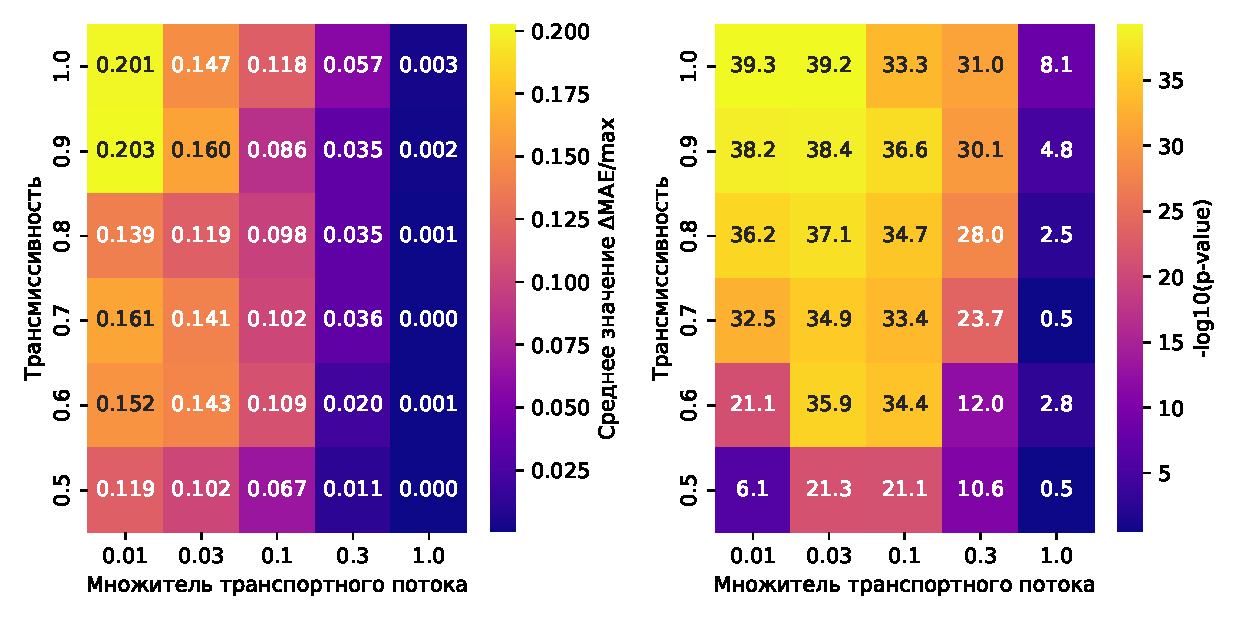
\includegraphics[width=\linewidth]{images/diffsatellites_heatmaps_mann.pdf}
    \caption{Тепловые карты средней разницы нормированных MAE эпидемиологических кривых (слева) и p-значения теста Манна-Уитни (справа).}
    \label{pic:diffsatellites_heatmaps}
\end{figure}

\newpage	
\subsection{Модель внутрироссийских авиаперелетов}

В данном эксперименте на основе географических данных о территориальных границах субъектов Российской Федерации и переписи населения 2021 года была создана транспортная модель, на которой были проведены эксперименты и анализ зависимости времени между пиками эпидемиологических кривых от логарифма величины транспортного потока.

Симуляция проводилась с числом агентов в 10 раз меньшем населения Российской Федерации для сокращения времени вычислений. Величины транспортных потоков рассчитывались из гравитационной модели, согласно которой поток между субъектами пропорционален произведению численностей их населений и обратно пропорционален расстоянию между ними к степени $1.5$. В качестве расстояния использовалось расстояние между геометрическими центрами субъектов, а не какими-либо конкретными городами. Калибровочная константа модели оценивалась на основе данных о годовом числе внутрироссийских пассажирских авиаперелетов и предположения о том, что в рассматриваемой модели все транспортные потоки определяются авиаперелетами. Были произведены вычисления для распространения эпидемии \gls{sars} при ее начале в Приморском крае и Москве.

На Рис. \ref{pic:country_map} приведены результаты симуляции. Цветом на карте показано отношение числа новых инфицирований на данном шаге симуляции к максимальному ее значению в ходе симуляции в рассматриваемом регионе. При начале эпидемии в Москве наблюдается волнообразное распространение инфекции из эпицентра. При начале в Приморском крае после завершения эпидемии в нем инфекционный агент появляется в большинстве субъектов практически одновременно. %Чукотский автономный округ остается неохваченным эпидемией ни в одном из экспериментов, так как в рассматриваемой модели обладает практически нулевыми транспортными потоками в абсолютной величине числа перемещаемых агентов в рассматриваемых масштабах числа агентов, уменьшенного в 10 раз по сравнению с реальными численностями населений.



 \begin{figure}[H]
    \centering
    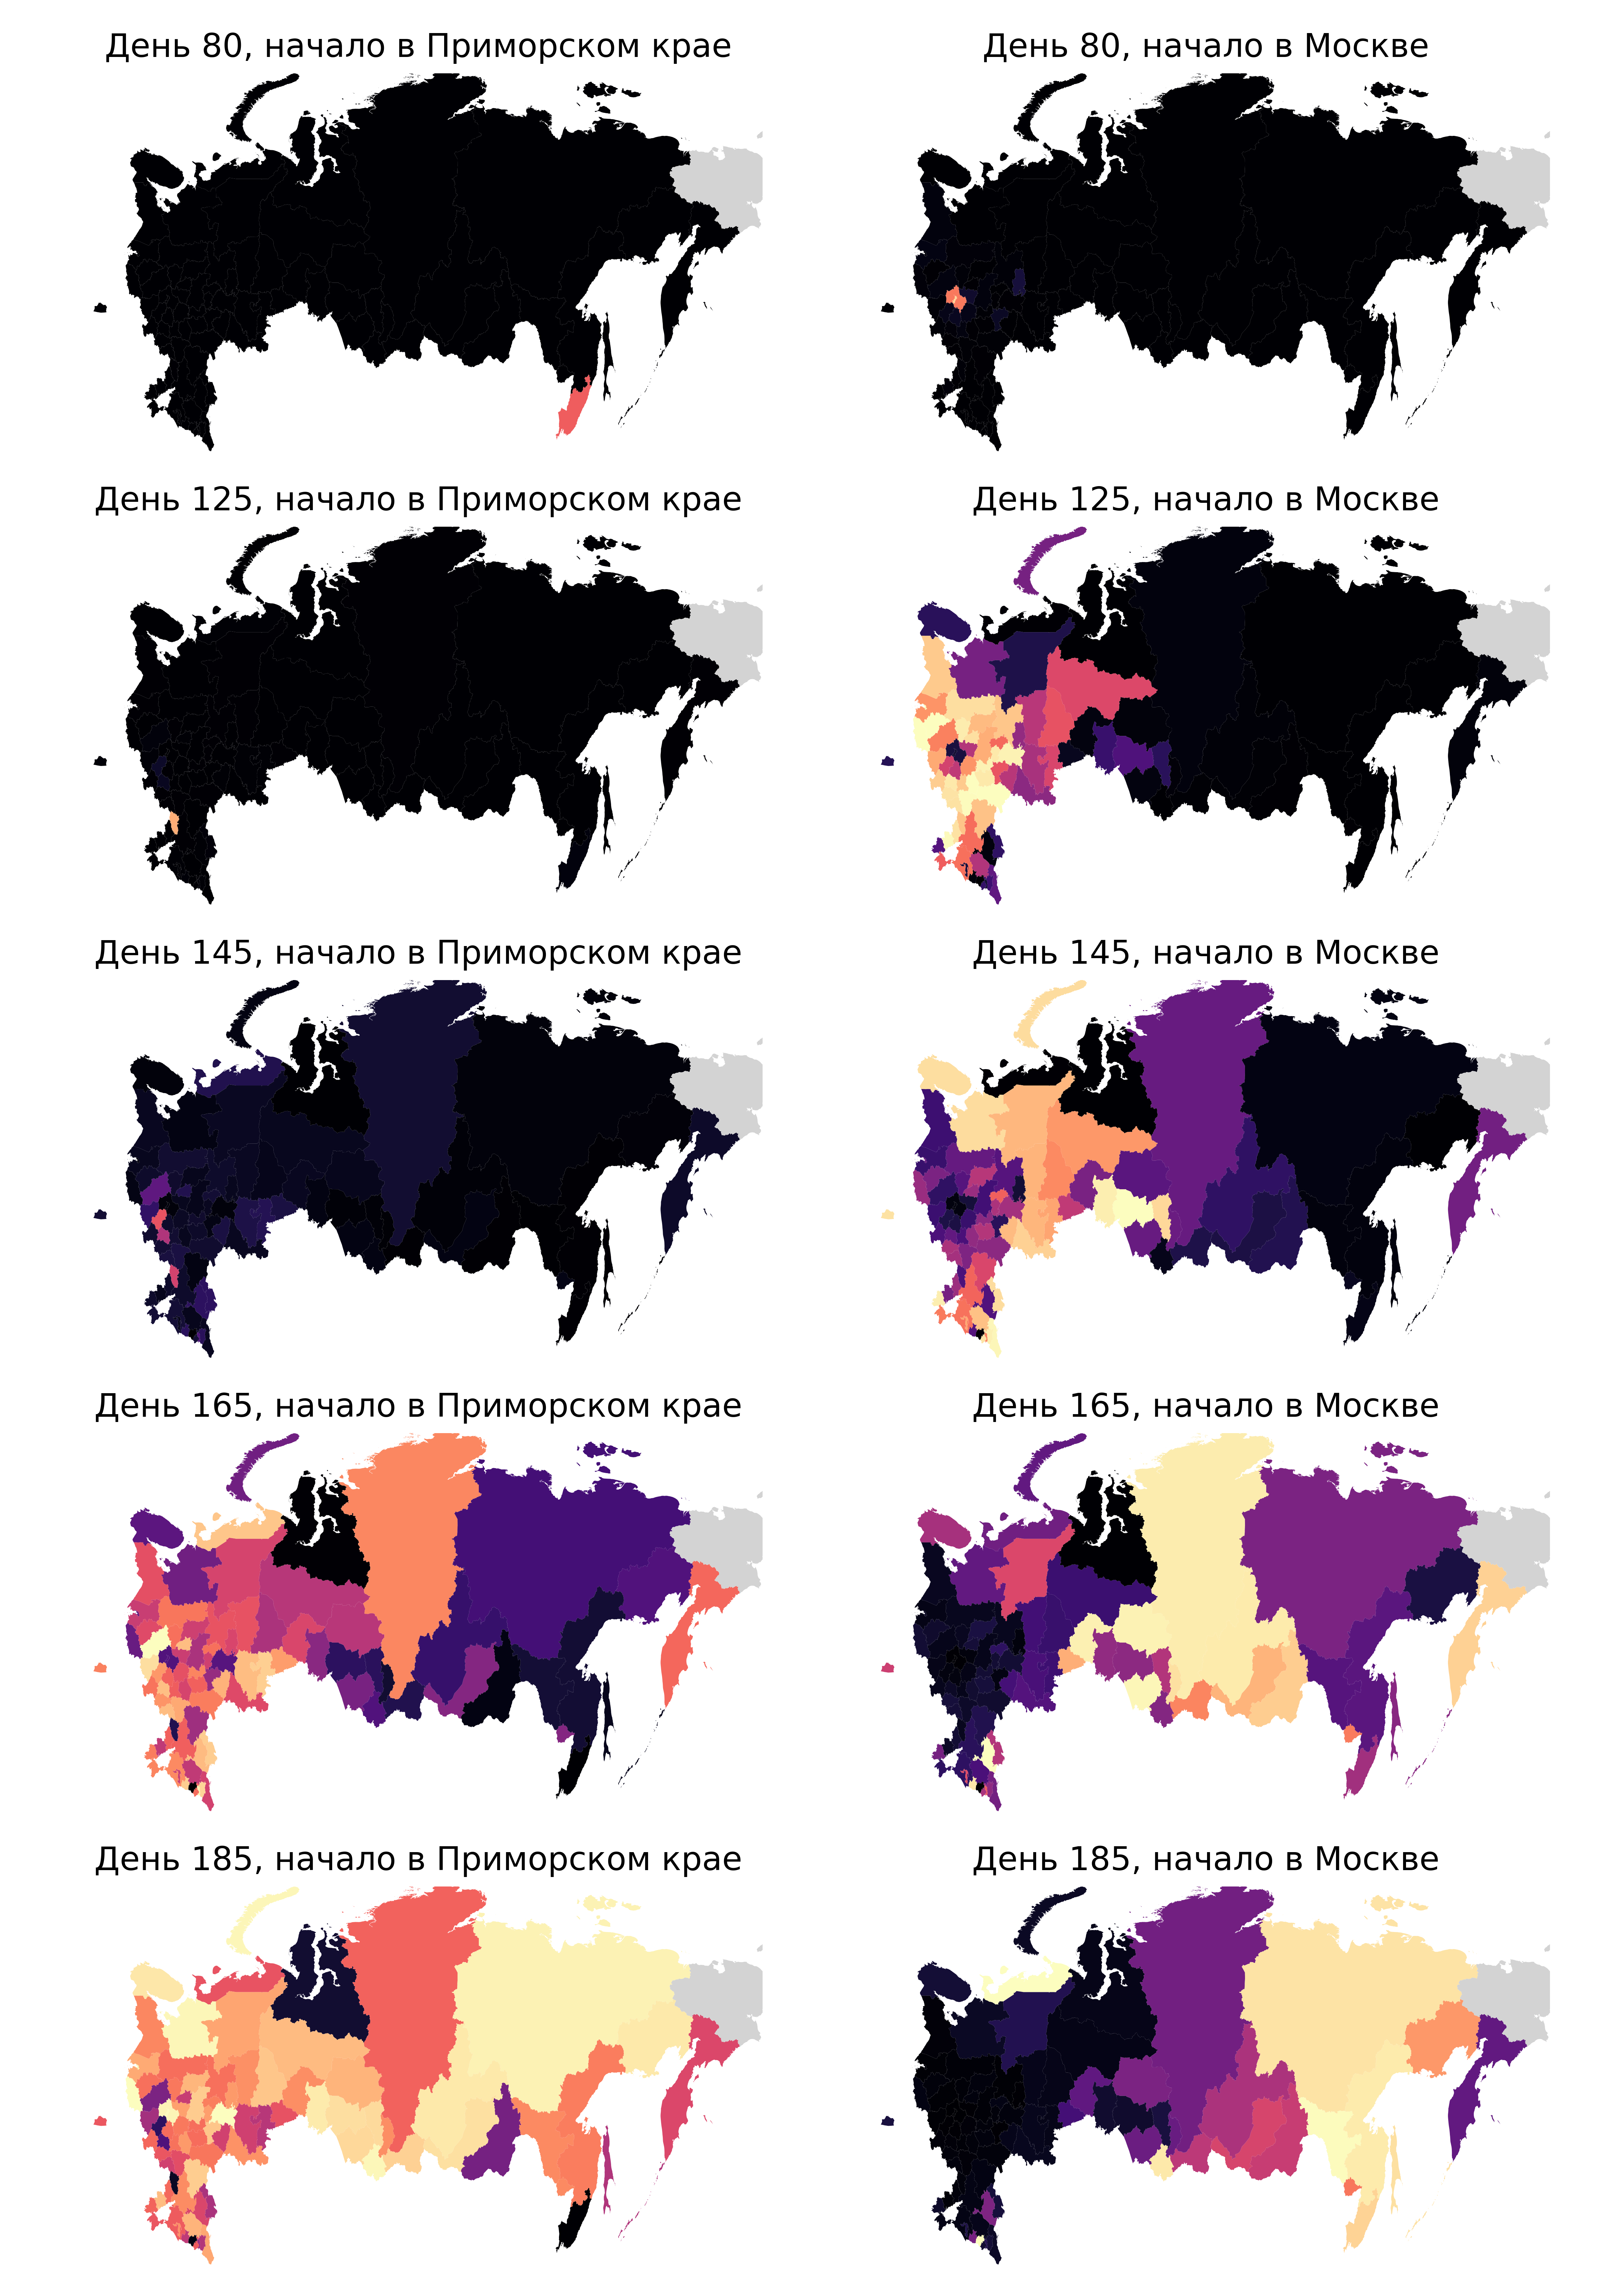
\includegraphics[width=\linewidth]{images/country_map.pdf}
    \caption{Ход развития эпидемии в модели транспортных потоков Российской Федерации при симуляции начала в Приморском крае (слева) и Москве (справа). Цветом обозначено отношение числа новых инфицирований на данном шаге симуляции к максимальному в рассматриваемом субъекте.}
    \label{pic:country_map}
\end{figure}


%Для проверки применимости в данном случае обнаруженной ранее линейной зависимости времени между пиками инфицирований от логарифма транспортного потока были построены графики соответствующих зависимостей. Также были построены графики аналогичных зависимостей для <<эффективных>> логарифмов потоков, полученных как сумма соответствующих логарифмов транспортных потоков при нахождении кратчайших расстояний в графах взаимодействий субъектов с помощью алгоритма Флойда-Уоршелла. 

%Оказывается, что такая модель достаточно хорошо описывает распространение инфекции при начале в Москве ($R^2=0.8$, с алгоритмом Флойда-Уоршелла $R^2=0.7$), но дает противоречивые результаты при начале в Приморском крае ($R^2=0.004$, с алгоритмом Флойда-Уоршелла $R^2=0.2$): угловой коэффициент полученной методом наименьших квадратов прямой положителен, что свидетельствует об увеличении задержки между пиками с увеличением транспортных потоков. Вероятно, наблюдаемый результат связан с тем, что в рассматриваемой гравитационной модели транспортные большинство величин транспортных потоков Приморского края одного порядка. Такого малого различия между потоками в логарифмическом масштабе оказывается недостаточно, чтобы преодолеть разброс результатов: среднеквадратичное отклонение разницы между днями пика эпидемии от линейной модели равном 10 дней, при этом при изменении величины транспортного потока на 1 порядок разница между днями пика меняется на 12 дней (для начала в Москве). Это подтверждает причину противоречивых результатов для Приморского края. Результаты приведены на Рис. \ref{pic:country_scatter}.


%\begin{figure}[H]
%    \centering
%    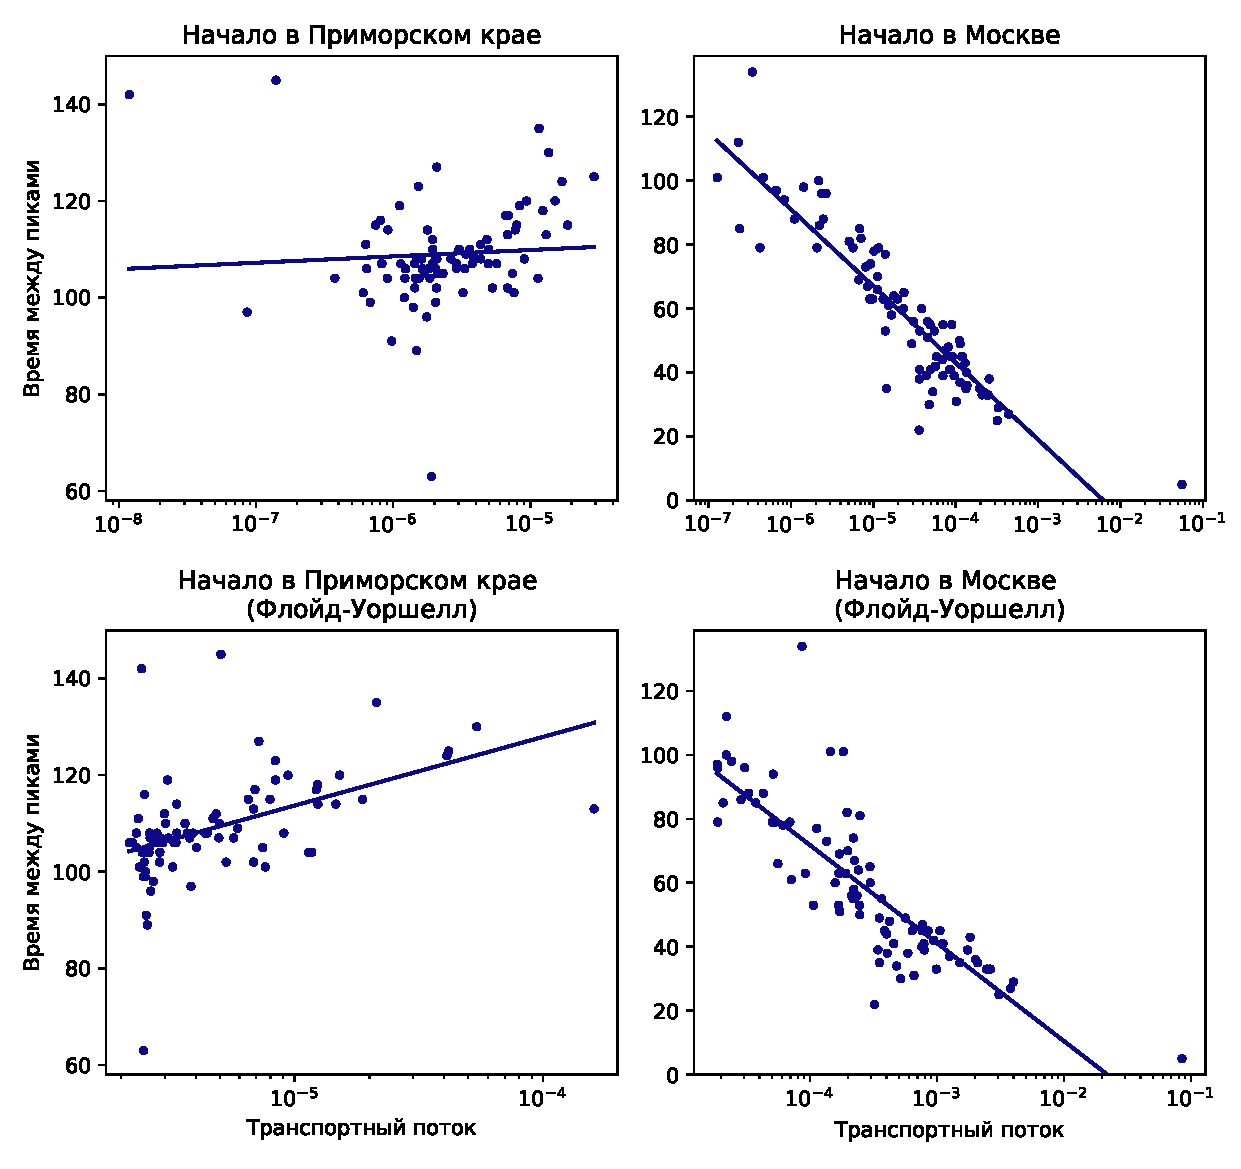
\includegraphics[width=\linewidth]{images/country_scatter.pdf}
%    \caption{Зависимости разницы между днями наступления пика эпидемии в субъекте и месте начала эпидемии (сверху) от величин транспортных потоков между ними в логарифмических координатах, зависимости от <<эффективных>> логарифмов потоков, полученных как сумма соответствующих логарифмов транспортных потоков при нахождении кратчайших расстояний в графах взаимодействий субъектов с помощью алгоритма Флойда-Уоршелла (снизу). Слева данные при начале эпидемии в Приморском крае, справа --- в Москве.}
%    \label{pic:country_scatter}
%\end{figure}



\section{Выводы}
В результате исследований в рамках данной работы были построены 3 модели транспортных потоков: модель системы двух городов, модель хаб-сателлиты, модель внутрироссийских авиаперелетов. После их исследования были получены следующие результаты.

Модель двух городов с одинаковой численностью агентов:
\begin{itemize}
\item[$\blacksquare$] Сдвиг эпидемиологической кривой эпидемии во втором городе относительно города начала есть монотонно убывающая функция трансмиссивности и транспортного потока, как и разброс результатов, и является линейной функцией логарифма величины транспортного потока;
\item[$\blacksquare$] t-статистика при сравнении средних дней наступления пика инфицирований монотонно возрастает с увеличением трансмиссивности, убывает с увеличением транспортного потока и является немонотонной выпуклой вверх функцией транспортного потока с максимумом при величине потока $< 10^{-4}$.
%\item[$\blacksquare$] При пороговом уровне значимости 0.05 при транспортных потоках не превышающих 0.003 наблюдается статистически значимая разница между временами наступления пиков инфицирований;
%\item[$\blacksquare$] Вычислены индексы чувствительности Соболя различных метрик эпидемии города начала и соседнего города к изменению транспортных потоков в системе при различных соотношениях между размерами популяций городов.
\end{itemize}

Модель хаб-сателлиты:
\begin{itemize}
\item[$\blacksquare$] Введение ограничений на транспортные потоки вплоть до
дня пика эпидемии позволяет достигнуть статистически значимого снижения пиковых
чисел инфицированных, критических случаев, смертей;
%\item[$\blacksquare$] При введении ограничений на главном
%плече эпидемии разница между уменьшением потоков в 10 и 100 раз между всеми
%городами или только между хабом и сателлитами незначительна. Проявляется она на ранних этапах эпидемии — там ограничения пассажиропотоков в 100 раз позволяют уменьшить пиковые значения еще
%практически в два раза в сравнении с введением на главном плече;
%\item[$\blacksquare$] Эффект от
%введения этих мер практически не меняется на главном плече эпидемии: удается достичь снижения пиковых чисел зараженных на $10\%$ ($p = 10^{-49}$), критических на $20\%$ ($p = 10^{-36}$), смертей на $20\%$ ($p = 10^{-25}$);
\item[$\blacksquare$] При начале эпидемии в сателлите ограничения только на потоки дорог, непосредственно связанных с этим сателлитом, значительно менее эффективны, чем ограничения на все потоки.
%\item[$\blacksquare$] При начале эпидемии в сателлите ключевой разницей является тот факт, что ограничения только на потоки дорог, непосредственно связанных с этим сателлитом, намного менее эффективны, чем ограничения на все потоки, хотя снижение целевых метрик и является статистически значимым.
%\item[$\blacksquare$] В подобной системе детектировать место начала эпидемии по стандартным метрикам (пиковое число зараженных, критических, мертвых, день пика инфицирований) не представляется возможным;
%\item[$\blacksquare$] Среднее значение разницы нормированных значений MAE при начале в хабе и сателлите
%есть монотонно убывающая функция множителя транспортного потока;
%\item[$\blacksquare$] t-статистика среднего значения разницы нормированных значений MAE при начале в хабе и сателлите является
%немонотонной выпуклой вверх функцией с максимумом вблизи множителя $3\cdot 10^{-2}$;
%\item[$\blacksquare$] По нормированному среднему значению MAE при пороговом уровне значимости 0.05 можно уверенно детектировать город начала эпидемии в такой системе для эпидемии уханьского штамма \gls{sars}, а при множителе на величины транспортных потоков меньше единицы и для эпидемий менее трансмиссивных инфекций.
\end{itemize}
%\item[!] Модель внутрироссийских авиаперелетов:
%\begin{itemize}
%\item[$\blacksquare$] При начале эпидемии в Москве линейная модель зависимости разницы между днями пиков инфицирований применима ($R^2=0.8$). Замена логарифма на <<эффективный>> поиском кратчайших расстояний в графе взаимодействий субъектов Российской Федерации алгоритмом Флойда-Уоршелла дает незначительную потерю качества модели ($R^2=0.7$);
%\item[$\blacksquare$] При начале эпидемии в Приморском крае линейная модель дает противоречивый результат в связи с недостаточной разницей его транспортных потоков для ее наблюдения на фоне шума. Поиск кратчайших расстояний не позволяет получить результат, согласующийся с реальностью.
%\end{itemize}

%\section{Благодарности}

\newpage
\printbibliography

\end{document}
